\documentclass[11pt]{article}
% Shared preamble for the GeoFDI theory notes.
\usepackage[T1]{fontenc}
\usepackage[utf8]{inputenc}
\usepackage{lmodern}
\usepackage[margin=1.1in]{geometry}
\usepackage{amsmath,amssymb,amsthm}
\usepackage{bm}
\usepackage{booktabs}
\usepackage{array}
\IfFileExists{microtype.sty}{\usepackage{microtype}}{}
\usepackage{xcolor}
\usepackage{tikz}
\usetikzlibrary{positioning,arrows.meta}
% todonotes needs TikZ; fall back to a plain red inline note if unavailable so
% the document still builds on a minimal TeX installation.
\IfFileExists{todonotes.sty}{%
  \usepackage[colorinlistoftodos,textsize=footnotesize]{todonotes}%
}{%
  \newcommand{\todo}[2][]{\textbf{\textcolor{red}{[TODO: #2]}}}%
  \newcommand{\listoftodos}{}%
}
% pending-anchor marker usable inside table cells (todonotes floats cannot live inside floats)
\newcommand{\pending}[1]{\textcolor{red!80!black}{[pending: #1]}}
\usepackage[colorlinks=true,linkcolor=blue!55!black,citecolor=blue!55!black,urlcolor=blue!55!black]{hyperref}

% ---------- theorem-like environments ----------
\newtheorem{theorem}{Theorem}[section]
\newtheorem{lemma}[theorem]{Lemma}
\newtheorem{proposition}[theorem]{Proposition}
\newtheorem{corollary}[theorem]{Corollary}
\newtheorem{conjecture}[theorem]{Conjecture}
\theoremstyle{definition}
\newtheorem{definition}[theorem]{Definition}
\newtheorem{example}[theorem]{Example}
\newtheorem{assumption}{Assumption}
\renewcommand{\theassumption}{A\arabic{assumption}}
\theoremstyle{remark}
\newtheorem{remark}[theorem]{Remark}

% ---------- notation macros ----------
\newcommand{\R}{\mathbb{R}}
\newcommand{\Law}{\operatorname{Law}}
\newcommand{\dtv}{d_{\mathrm{TV}}}
\newcommand{\SE}{\mathrm{SE}}
\newcommand{\SO}{\mathrm{SO}}
\newcommand{\Ogrp}{\mathrm{O}}
\newcommand{\eqdist}{\overset{d}{=}}
\newcommand{\gs}{g_{\mathrm{s}}}               % sagittal reflection
\newcommand{\symgrp}{\Sigma}                   % spatio-temporal gait symmetry group
\newcommand{\eps}[1]{\varepsilon_{\mathrm{#1}}}          % per-transition equivariance defect (A1'-A4')
\newcommand{\epsbar}[1]{\bar\varepsilon_{\mathrm{#1}}}   % cycle-level defect (Definition def:cycle-eps)
\newcommand{\Tc}{T_{\mathrm{c}}}                          % closed-loop transition steps per gait cycle
\newcommand{\repQ}{\rho_{Q}}
\newcommand{\repX}{\rho_{X}}
\newcommand{\repU}{\rho_{U}}
\newcommand{\repY}{\rho_{Y}}
\newcommand{\repR}{\rho_{R}}
\newcommand{\repW}{\rho_{W}}                   % block action on the data space W = X x U x Y
\newcommand{\repenv}{\rho_{\mathrm{env}}}      % action on exogenous environment inputs
\newcommand{\push}[1]{{#1}_{\#}}               % pushforward of a measure


\title{GeoFDI Theory Notes --- Parts 0--2:\\ Hypotheses and Assumptions; Exactness and Isotypic Detectability (core);\\ Residual Data Elements and Equivariant Nominal Models}
\author{GeoFDI project}
\date{August 15, 2026 --- working notes: Part 0 v1.2, Part 1 core (Sprint-6 stand-in), Part 2 v1}

\begin{document}
\maketitle

\begin{abstract}
We formalize the null hypothesis underlying GeoFDI: for a legged robot whose
morphology, controller, environment, and sensing are (approximately) symmetric,
the phase-registered per-cycle data stream is distribution-invariant under the
gait's spatio-temporal symmetry group $\symgrp \subset G \times S^1$. Faults
that break this symmetry become detectable as violations of distributional
invariance, without any dynamics model of the fault. This note fixes notation
and the concrete form of the symmetry representations (including the
pseudovector transformation of gyroscope channels), states the standing
assumptions A1--A5 with $\varepsilon$-approximate variants, audit procedures,
and degradation paths, and derives the hypotheses $H_0$ and $H_1$, an
$\varepsilon$-robustness lemma, and the recalibrated null $H_0'$ used when
exact controller symmetry fails (Part~0). A minimal Part~1 core states the
exactness of the flip test and the isotypic characterization of what an
invariance test can detect. Part~2 makes the residual of a nominal model a
legitimate data element: an equivariant nominal model (analytic observer or
a Deep Lagrangian Network made exactly equivariant by mirror weight sharing)
passes $H_0$ from the data to the residual, so the same exact test acts on
$\Pi^{-}r$ while the magnitude channel reads $\Pi^{+}r$; a non-equivariant
model contaminates $H_0$ by a fifth $\varepsilon$-term controlled by its
equivariance defect; and the residual channel dominates the raw-signal
channel in power under an explicit signal-to-noise condition.
\end{abstract}

\tableofcontents
\listoftodos

\section{Scope and notation}
\label{sec:notation}

These notes are Part~0 of the GeoFDI theory series. They fix notation and the
concrete form of the symmetry representations, state the standing assumptions
\ref{as:dyn}--\ref{as:erg} together with $\varepsilon$-approximate variants,
audit procedures, and degradation paths, and formalize the null hypothesis
$H_0$ (distributional symmetry of healthy gait data), the structured
alternative $H_1$, and the recalibrated null $H_0'$. Test construction,
cross-cycle exchangeability, the isotypic detectability characterization, and
full proofs are deferred to later parts (workstreams N1-1 through N1-4).

The project sits between two literatures. Model-based proprioceptive fault and
collision detection builds residuals from a dynamics model and monitors them
\cite{haddadin2017robot,evangelisti2024datadriven}; symmetry-aware robotics
identifies the finite morphological symmetry group of a robot and exploits it
as an algebraic structure on models and data
\cite{ordonez2023discrete,ordonez2025morphological}. GeoFDI uses the second
structure to stand in for the first's model: under the assumptions of
Section~\ref{sec:assumptions}, \emph{healthy} closed-loop gait data is
distribution-invariant under the gait's spatio-temporal symmetry group, so
fault detection reduces to statistical testing of group invariance --- a
hypothesis class that admits exact, distribution-free permutation tests
\cite{hemerik2018exact} and anytime-valid sequential e-processes
\cite{perezortiz2024estatistics}.

\subsection{State, input, output, and residual spaces}
\label{sec:spaces}

We consider a floating-base legged robot with $n_j$ actuated joints. The
configuration space is
\[
  Q \;=\; \SE(3) \times \mathbb{T}^{n_j},
  \qquad q = (q_B, q_J),
\]
with $q_B = (R_{B}, p_{B}) \in \SE(3)$ the base pose (body-to-world rotation
and world position) and $q_J \in \mathbb{T}^{n_j}$ the joint coordinates. The
state is $x = (q, v) \in X = TQ$, where $v = (\xi, \dot q_J) \in \R^{6+n_j}$
stacks the body twist $\xi = (v_b, \omega_b)$ and the joint rates. Actuation
commands (desired torques or motor commands) live in $u \in U \subseteq
\R^{n_u}$. The measured output $y \in Y$ collects the proprioceptive channels:
IMU specific force $a$ and angular rate $\omega$, joint encoders and rates,
motor currents or measured torques, and per-leg contact indicators
$c \in \{0,1\}^{4}$.

A \emph{residual} $r \in R$ is any causally computed function of the data
stream designed to be small or structured when the robot is healthy. The
theory below treats $y$ and $r$ generically; the concrete channels planned for
GeoFDI are the innovation sequences of a contact-aided invariant extended
Kalman filter \cite{hartley2020contact,barrau2017invariant} and
generalized-momentum residuals \cite{evangelisti2024datadriven}, alongside raw
tracking errors. When a residual generator is built equivariantly, the induced
representation $\repR$ on $R$ makes the residual stream inherit the symmetry
of the data (workstream N2).

\subsection{Morphological symmetry group and representations}
\label{sec:group}

$G$ denotes the finite morphological symmetry group of the robot: the group of
transformations that map the mechanism onto itself (relabeling mirrored limbs
and reflecting spatial quantities) while preserving its kinematic and dynamic
description \cite{ordonez2023discrete,ordonez2025morphological}. $G$ acts on
every space in play through representations
\[
  \repQ \text{ on } Q,\qquad
  \repX \text{ on } X,\qquad
  \repU \text{ on } U,\qquad
  \repY \text{ on } Y,\qquad
  \repR \text{ on } R,
\]
whose concrete matrices are spelled out in Section~\ref{sec:reps}. A map
$h : X \times U \to X$ is \emph{$G$-equivariant} if
$h(\repX(g)x, \repU(g)u) = \repX(g)\,h(x,u)$ for all $g \in G$. We write
$W = X \times U \times Y$ for the per-sample data space and
$\repW = \repX \oplus \repU \oplus \repY$ for the block action on it.
Exogenous environment inputs (terrain heights, pushes) are denoted
$w$ with action $\repenv$.

\begin{table}[ht]
\centering
\small
\begin{tabular}{@{}ll@{}}
\toprule
symbol & meaning \\
\midrule
$Q = \SE(3)\times\mathbb{T}^{n_j}$ & configuration space: floating base $\times$ joints \\
$x = (q,v) \in X$ & state; $v = (\xi, \dot q_J)$ body twist and joint rates \\
$u \in U$ & actuation commands (torques / motor commands) \\
$y \in Y$ & proprioceptive outputs (IMU, encoders, currents, contacts) \\
$r \in R$ & residual channels (InEKF innovations, momentum residuals, \dots) \\
$G$, $\gs$ & finite morphological symmetry group; sagittal reflection ($G=\mathbb{C}_2$ for M1) \\
$\repQ,\repX,\repU,\repY,\repR$ & representations of $G$ on the respective spaces \\
$W$, $\repW$ & data space $X\times U\times Y$ and its block action \\
$w$, $\repenv$ & exogenous environment inputs and their action \\
$\theta \in S^1 = \R/\mathbb{Z}$ & gait phase (period normalized to 1); $T$ = period [s] \\
$\symgrp \subset G \times S^1$ & spatio-temporal symmetry group of the commanded gait \\
$\sigma = (g, \Delta\theta)$ & element of $\symgrp$: spatial action paired with phase shift \\
$Z_k$ & phase-registered per-cycle data element, cycle $k$ \\
$\rho(\sigma)$ & action on cycle elements: $(\rho(\sigma)Z)(\theta) = \repW(g)\,Z(\theta+\Delta\theta)$ \\
$\eps{dyn},\eps{ctrl},\eps{env},\eps{noise}$ & per-transition equivariance defects (A1$'$--A4$'$) \\
$\epsbar{dyn},\epsbar{ctrl},\epsbar{env},\epsbar{noise}$ & cycle-level defects (Definition~\ref{def:cycle-eps}) \\
$\Tc$ & closed-loop transition steps per gait cycle \\
$\nu$, $\nu_0$ & asymmetry functional and its calibration value (for $H_0'$) \\
\bottomrule
\end{tabular}
\caption{Symbols used throughout the GeoFDI notes.}
\label{tab:symbols}
\end{table}

\subsection{Gait phase and per-cycle data elements}
\label{sec:cycles}

The commanded gait is periodic with period $T$; the \emph{gait phase}
$\theta(t) \in S^1$ is the normalized position within the cycle, estimated from
contact events or a phase oscillator (workstream N1/N3; the phase-registration
error budget enters the $\varepsilon$ accounting of
Section~\ref{sec:h0prime}). Slicing the telemetry at phase zero yields the
\emph{per-cycle data element}
\[
  Z_k \;=\; \bigl\{\, (x(t), u(t), y(t)) \;:\; t \in \text{cycle } k \,\bigr\},
\]
which after phase registration is a random function
$Z_k : S^1 \to W$ --- the fundamental statistical object of this project: all
tests act on the sequence $(Z_k)_{k\ge 1}$, never on raw time series.%
\footnote{In implementation, channels are resampled on a fixed $N$-point phase
grid, so $Z_k$ is a random vector in $\R^{dN}$ ($d$ channels); every law below
lives on that finite-dimensional space, which sidesteps measure-theoretic
subtleties on function spaces. $N$ is a protocol parameter.}

For $\sigma = (g, \Delta\theta) \in G \times S^1$ define the action on cycle
elements by
\begin{equation}
  \label{eq:cycle-action}
  (\rho(\sigma) Z)(\theta) \;=\; \repW(g)\, Z(\theta + \Delta\theta),
\end{equation}
i.e.\ spatially transform every channel and shift the phase. This is a group
action, and restricting it to the gait's symmetry group $\symgrp$
(Section~\ref{sec:gait}) gives the invariance tested by $H_0$.

\subsection{Concretization for the M1 quadruped}
\label{sec:m1}

For the M1 quadruped we take
\[
  G \;=\; \mathbb{C}_2 \;=\; \{e, \gs\},
\]
where $\gs$ is the sagittal (left--right) reflection, acting on leg labels by
the permutation
\[
  \sigma_{\mathrm{s}} \;=\; (\mathrm{LF}\;\mathrm{RF})(\mathrm{LH}\;\mathrm{RH}),
\]
i.e.\ left-front $\leftrightarrow$ right-front and left-hind
$\leftrightarrow$ right-hind. Front--hind symmetry is \emph{not} assumed (mass
distribution and leg geometry differ between front and hind pairs), so the
richer groups $\mathbb{C}_2\times\mathbb{C}_2$ or $\mathbb{K}_4$ of idealized
quadrupeds are unavailable.

\paragraph{Joint count, ordering and reflection signs (resolved on hardware).}
The M1 platform is a \emph{wheeled-legged} quadruped: $n_j = 16$, four legs
$\times$ (ABAD = hip roll, HIP = hip pitch, KNEE = knee pitch, WHEEL). The
ordering and every reflection sign in Table~\ref{tab:joint-signs} were fixed on
the 2026-08-10 hardware corpus (\texttt{docs/protocol/m1\_h\_data\_audit.md};
telemetry names \texttt{fl1\_hip\_roll \dots br4\_foot}), superseding the
placeholder that stood here.

Two conventions must be kept apart. In the \emph{uniform-axis} convention used
throughout this document, a channel's mirror sign is decided by whether it is a
polar or an axial quantity about the sagittal plane: the roll-axis joint flips,
the pitch-axis joints do not. In the \emph{vendor} frame the manufacturer may
already define mirrored positive directions, in which case the raw telemetry
carries extra sign flips that the loader must undo before the representation
$\repW(\gs)$ of \eqref{eq:cycle-action} applies --- this is the case for M1,
where all four joints flip between mirror legs in vendor coordinates.

\begin{table}[ht]
\centering
\footnotesize
\begin{tabular}{@{}p{2.6cm}p{3.5cm}p{2.5cm}cc@{}}
\toprule
platform & channel & kind & $\repW(\gs)$ & vendor$\to$uniform (R legs) \\
\midrule
M1 (16 joints) & ABAD (hip roll) & axial-about-$x$ & $-1$ & $+1$ \\
               & HIP (hip pitch) & pitch axis & $+1$ & $-1$ \\
               & KNEE (knee pitch) & pitch axis & $+1$ & $-1$ \\
               & WHEEL (rate) & pitch axis & $+1$ & $-1$ \\
\midrule
Go2 (no joints) & \texttt{foot\_pos}/\texttt{foot\_vel} $(x,y,z)$ & polar vector & $(+1,-1,+1)$ & --- \\
               & \texttt{foot\_force} & magnitude & $+1$ & --- \\
\midrule
both & IMU accelerometer & polar & $\operatorname{diag}(+1,-1,+1)$ & --- \\
     & IMU gyroscope & axial & $\operatorname{diag}(-1,+1,-1)$ & --- \\
\bottomrule
\end{tabular}
\caption{Per-channel reflection signs under $\gs$, verified on hardware. M1:
Sprint~8 audit; the wheel \emph{angle} is unbounded (the vendor wraps it to
$[-\pi,\pi)$) and is therefore excluded from the data element, while the wheel
\emph{rate} and torque stay. The rightmost column is the extra flip the loader
applies to the right legs to leave the vendor frame; the forward-rolling sign of
the wheel is additionally $-1$ on the left legs and $+1$ on the right. Go2
(Sprint~9): the high-level API exposes \emph{no} joint stream, so the element is
built from the robot's own forward kinematics
(\texttt{foot\_position\_body}/\texttt{foot\_speed\_body}) plus foot force and
the IMU; the same $\mathbb{C}_2$ representation applies channel-wise.}
\label{tab:joint-signs}
\end{table}

For the Go2 corpus of Sprint~9 the situation is different in kind rather than in
degree: the recorded high-level interface (\texttt{SportModeState}) carries no
\texttt{motorState}, so $n_j$ is not observable at all. What it does publish is
the manufacturer's own forward kinematics of each leg, which is a bijective
re-coordinatisation of the leg joint vector, so the mirror pairing and the
isotypic split of Section~\ref{sec:reps} go through unchanged on those channels.
Only the torque channel --- and with it the model-residual ($R^+$) layer --- is
lost.

\section{Hypotheses and standing assumptions}
\label{sec:assumptions}

This section is written to be liftable into the paper's appendix. Throughout,
``nominal'' means fault-free hardware executing the commanded gait;
``healthy law'' means the probability law of the nominal per-cycle elements
$Z_k$ of Section~\ref{sec:cycles}.

\subsection{Concrete form of the morphological representations}
\label{sec:reps}

Fix the world frame with $x$ forward, $y$ to the robot's left, $z$ up, so the
sagittal plane is the $x$--$z$ plane. The sagittal reflection acts on
$\R^3$ by
\[
  E \;=\; \operatorname{diag}(1,-1,1) \;\in\; \Ogrp(3),
  \qquad \det E = -1,\qquad E^2 = I .
\]

\paragraph{Base pose.}
On the base pose $q_B = (R_B, p_B) \in \SE(3)$ the reflection acts by the
conjugation
\begin{equation}
  \label{eq:base-action}
  \repQ(\gs)\,(R_B,\, p_B) \;=\; \bigl(E\,R_B\,E,\;\; E\,p_B\bigr).
\end{equation}
Conjugating (rather than left-multiplying) keeps the result in $\SO(3)$:
$\det(E R_B E) = \det R_B = +1$. Geometrically, the mirrored robot's body
frame is itself reflected, which restores right-handedness; this is the
standard action of reflections on floating-base systems
\cite{ordonez2025morphological}.

\paragraph{Base velocities.}
Body-frame linear velocity is a true (polar) vector, body-frame angular
velocity is a pseudovector (axial vector):
\begin{equation}
  \label{eq:twist-action}
  v_b \;\longmapsto\; E\,v_b,
  \qquad
  \omega_b \;\longmapsto\; \det(E)\,E\,\omega_b \;=\; -E\,\omega_b .
\end{equation}
Since $-E = \operatorname{diag}(-1,1,-1)$, the pitch rate $\omega_y$ is
\emph{preserved} while roll $\omega_x$ and yaw $\omega_z$ \emph{flip} --- as
intuition demands: a robot rolling to its left maps to one rolling to its
right, while pitching forward stays pitching forward.

\paragraph{Joint coordinates.}
The reflection permutes legs by $\sigma_{\mathrm{s}}$ and flips the sign of
joints whose axes are reversed by the mirror. With three joints per leg
(hip abduction/adduction HAA, hip flexion/extension HFE, knee KFE) and the
\emph{uniform-axis convention} (all four legs carry identically oriented joint
axes), the joint representation is
\begin{equation}
  \label{eq:joint-action}
  q_J \;\longmapsto\; P_{\gs}\, q_J,
  \qquad
  P_{\gs} \;=\; \Pi_{\sigma_{\mathrm{s}}} \otimes S,
  \qquad
  S = \operatorname{diag}(s_{\mathrm{HAA}}, s_{\mathrm{HFE}}, s_{\mathrm{KFE}}),
\end{equation}
where $\Pi_{\sigma_{\mathrm{s}}}$ is the $4\times4$ leg-permutation matrix and
the signs follow from the axis directions (Table~\ref{tab:joint-signs}).

\begin{table}[ht]
\centering
\small
\begin{tabular}{@{}llll@{}}
\toprule
joint & axis (uniform convention) & behavior under $\gs$ & sign $s$ \\
\midrule
hip abduction/adduction (HAA, ``roll'')   & $\pm x$ & leg swapped, angle flips & $-1$ \\
hip flexion/extension (HFE, ``pitch'')    & $\pm y$ & leg swapped, angle kept  & $+1$ \\
knee flexion/extension (KFE, ``pitch'')   & $\pm y$ & leg swapped, angle kept  & $+1$ \\
wheel spin (if present)                   & $\pm y$ & leg swapped, rate kept   & $+1$ \\
\bottomrule
\end{tabular}
\caption{Per-joint transformation under the sagittal reflection, assuming the
uniform-axis convention. The M1-specific signs are to be \emph{measured}, not
assumed (see the remark below).}
\label{tab:joint-signs}
\end{table}

\begin{remark}[Vendor conventions absorb signs]
\label{rem:vendor-signs}
Firmware and URDF files frequently define \emph{mirrored} positive directions
between left and right legs, in which case part or all of $S$ is absorbed into
the coordinates and $P_{\gs}$ is closer to a pure permutation. The actual $S$
for M1 must therefore be established from data (commanding small symmetric
motions and checking recorded signs), not read off a datasheet.
\todo[inline]{Back-fill the M1 joint ordering, per-joint signs, and wheel DoFs
(if any) in Table~\ref{tab:joint-signs} after the Day-0 telemetry audit.}
\end{remark}

\paragraph{Actuation.}
Joint torques are conjugate to joint coordinates and transform by the same
matrix: $\repU(\gs) = P_{\gs}$ (restricted to the actuated coordinates).
Signed motor currents follow the torque sign; magnitude-only channels
(e.g.\ RMS current, temperature) transform by the pure permutation
$\Pi_{\sigma_{\mathrm{s}}}$.

\paragraph{IMU channels.}
The accelerometer measures specific force, a true vector; the rate gyro
measures angular velocity, a pseudovector:
\begin{equation}
  \label{eq:imu-action}
  a \;\longmapsto\; E\,a,
  \qquad
  \omega \;\longmapsto\; \det(E)\,E\,\omega \;=\; -E\,\omega .
\end{equation}
(A magnetometer, if one is ever used, measures the magnetic field --- also a
pseudovector --- and transforms like $\omega$.)%
\footnote{This sign is a known implementation trap: applying $E$ instead of
$-E$ to the gyro corrupts the mirrored data by a sign error on the
$\omega_x,\omega_z$ (equivalently, on $\omega_y$, depending on the erroneous
variant) channels, so mirrored and original healthy data \emph{systematically}
disagree. The test then rejects $H_0$ on a perfectly healthy robot ---
symmetry breaking fabricated by software, indistinguishable from a real fault
and not fixable by more data. Guard: unit-test all representation code on
simulated trajectories mirrored analytically, where invariance is exact by
construction.}

\paragraph{Contacts and ground reactions.}
Per-leg contact indicators are permuted without signs:
$c \mapsto \Pi_{\sigma_{\mathrm{s}}}\, c$. World-frame ground reaction forces
are true vectors attached to legs, $f_i \mapsto E\, f_{\sigma_{\mathrm{s}}(i)}$;
contact torques, if measured, are pseudovectors,
$\tau_i \mapsto -E\, \tau_{\sigma_{\mathrm{s}}(i)}$.

Collecting the blocks above gives the explicit matrices of
$\repX$, $\repU$, $\repY$; the residual representation $\repR$ is induced by
the (equivariant) residual generator (workstream N2).

\subsection{Spatio-temporal gait symmetry}
\label{sec:gait}

A periodic gait couples space and time: reflecting a trotting robot does not
reproduce the same instantaneous picture --- it reproduces the picture
\emph{half a period later}. The right symmetry object is therefore not $G$
alone but a subgroup of $G \times S^1$
\cite{golubitsky1999symmetry,collins1993coupled,golubitsky2002symmetry}.

\begin{definition}[Gait symmetry group]
\label{def:gait-group}
The commanded gait prescribes a subgroup
$\symgrp \subset G \times S^1$, the \emph{spatio-temporal symmetry group} of
the gait. The nominal closed-loop process is called $\symgrp$-symmetric if for
every $\sigma = (g, \Delta\theta) \in \symgrp$ and all $t$,
\begin{equation}
  \label{eq:st-symmetry}
  \bigl(x(t + \Delta\theta\, T),\; u(t + \Delta\theta\, T)\bigr)
  \;\eqdist\;
  \bigl(\repX(g)\, x(t),\; \repU(g)\, u(t)\bigr),
\end{equation}
with $\eqdist$ denoting equality in distribution.
\end{definition}

\paragraph{Trot.}
The symmetric trot pairs diagonal legs and is generated by the single element
$\sigma_* = (\gs, \tfrac12)$:
\begin{equation}
  \label{eq:trot}
  \Bigl(x\bigl(t+\tfrac{T}{2}\bigr),\; u\bigl(t+\tfrac{T}{2}\bigr)\Bigr)
  \;\eqdist\;
  \bigl(\repX(\gs)\,x(t),\; \repU(\gs)\,u(t)\bigr),
\end{equation}
i.e.\ \emph{reflection composed with a half-period shift} --- not a pure
spatial reflection. Since $\Delta\theta = \tfrac12$ is 2-torsion in $S^1$,
$\sigma_*^2 = (e, 0)$ and $\symgrp_{\mathrm{trot}} = \{(e,0), (\gs,\tfrac12)\}
\cong \mathbb{Z}_2$.

\paragraph{Contrast: pronk and walk.}
Two bracketing examples fix intuition:
\begin{itemize}
  \item \emph{Pronk} (all four legs in phase): the symmetry element is
  $(\gs, 0)$ --- pure spatial reflection with \emph{zero} shift.
  \item \emph{Walk}: primary walking gaits carry a \emph{quarter-period}
  structure --- legs fire in sequence with $\Delta\theta = \tfrac14$ spacing,
  and the full spatio-temporal symmetry is a cyclic group of order four
  generated by a leg-cycling permutation with a $\tfrac14$ shift
  \cite{golubitsky1999symmetry,collins1993coupled}. Leg-cycling permutations
  mix front and hind legs, however, and are morphological symmetries only when
  $G$ is larger than the sagittal $\mathbb{C}_2$. With $G = \mathbb{C}_2$
  (the M1 case), the usable element of a lateral-sequence walk --- legs at
  phases $\mathrm{LF}\!:0$, $\mathrm{RH}\!:\tfrac14$, $\mathrm{RF}\!:\tfrac12$,
  $\mathrm{LH}\!:\tfrac34$ --- is again $(\gs, \tfrac12)$, since each mirror
  pair sits half a period apart.
\end{itemize}

\begin{definition}[Mirror-pairing rule]
\label{def:pairing}
Let $\symgrp$ be generated by $(g, \Delta\theta_{\mathrm{gait}})$. Every
scalar channel attached to leg $i$ and registered at phase $\theta$ is paired
with the same channel of leg $\sigma(i)$ at phase
$\theta + \Delta\theta_{\mathrm{gait}}$, after multiplication by the channel's
sign under $\rho(g)$ (Section~\ref{sec:reps}). Under $H_0$
(Definition~\ref{def:h0}) paired quantities are equal in distribution.
\end{definition}

Definition~\ref{def:pairing} is the construction rule for \emph{every} test
statistic in this project: mirror pairs are the atoms from which paired
differences, rank statistics, and kernel two-sample statistics are built. For
the M1 trot: leg LF at phase $\theta$ pairs with leg RF at phase
$\theta + \tfrac12$, and leg LH at $\theta$ with RH at $\theta + \tfrac12$.

\subsection{Standing assumptions A1--A4}
\label{sec:standing}

Each assumption is stated in four registers: exact statement,
$\varepsilon$-approximate variant (in total-variation distance), audit (who
verifies it, on which data), and degradation path if falsified.

\paragraph{Kernel notation.}
The sampled nominal closed loop factorizes into a dynamics transition kernel
$P_{\mathrm{dyn}}(\mathrm{d}x^+ \mid x, u, w)$, a (possibly randomized) policy
kernel $P_{\mathrm{ctrl}}(\mathrm{d}u \mid x, \theta)$, an exogenous
environment law $P_{\mathrm{env}}$ (terrain field and disturbances over a
cycle), and an observation kernel $P_{\mathrm{obs}}(\mathrm{d}y \mid x)$. For
a measurable map $\rho$ and a measure $\mu$, $\push{\rho}\mu$ denotes the
pushforward; $\dtv$ is total variation; $\mathcal{K}$ is a compact operating
region (the states, inputs, and environments visited by the commanded gait
class). All suprema below are over $\mathcal{K}$.

% ---------------------------------------------------------------- A1
\begin{assumption}[Dynamics $G$-equivariance]
\label{as:dyn}
The nominal dynamics is $G$-equivariant: the drift satisfies
$f(\repX(g)x, \repU(g)u) = \repX(g) f(x,u)$ for all $g \in G$, and, including
process noise and exogenous inputs, the transition kernel satisfies
\[
  \push{\repX(g)}\, P_{\mathrm{dyn}}(\cdot \mid x, u, w)
  \;=\;
  P_{\mathrm{dyn}}\bigl(\cdot \mid \repX(g)x,\, \repU(g)u,\, \repenv(g)w\bigr)
  \qquad \forall g \in G .
\]
\end{assumption}

\emph{$\varepsilon$-variant (A1$'$).} The defect
\[
  \eps{dyn}
  \;=\;
  \sup_{(x,u,w) \in \mathcal{K},\; g \in G}
  \dtv\Bigl(
    \push{\repX(g)}\, P_{\mathrm{dyn}}(\cdot \mid x,u,w),\;
    P_{\mathrm{dyn}}\bigl(\cdot \mid \repX(g)x, \repU(g)u, \repenv(g)w\bigr)
  \Bigr)
\]
is finite and small.

\emph{Nature and audit.} A1 is the structural morphological-symmetry
assumption: it follows from a symmetric kinematic tree and symmetric mass
distribution \cite{ordonez2023discrete,ordonez2025morphological}.
Manufacturing asymmetry (mass and CoM offsets, friction spread, belt tension)
makes exact equality false on real hardware; those effects are \emph{folded
into $\eps{dyn}$}, not treated as faults. Audit: URDF/CAD parameter
comparison plus mirrored system identification on \texttt{raw/m1/audit}
sessions (per-joint chirps, slow sinusoids); statistic: relative gap between
mirror-leg identified parameters.

\emph{Degradation if falsified.} Per-leg nominal bias calibration: learn
per-leg reference offsets during a certified-healthy calibration window and
subtract them before testing --- i.e.\ absorb the \emph{static} part of the
asymmetry into the reference measure, leaving only the dynamic part in
$\eps{dyn}$. (Operationally this coincides with moving toward $H_0'$,
Section~\ref{sec:h0prime}.)

% ---------------------------------------------------------------- A2
\begin{assumption}[Controller equivariance --- empirical, not axiomatic]
\label{as:ctrl}
The closed-loop policy $\pi$ respects the gait symmetry: for all
$\sigma = (g, \Delta\theta) \in \symgrp$,
\[
  \pi\bigl(\repX(g)\,x,\; \theta\bigr)
  \;=\;
  \repU(g)\,\pi\bigl(x,\; \theta + \Delta\theta\bigr),
\]
and, for randomized or filtered controllers, the policy kernel satisfies the
corresponding distributional identity
$\push{\repU(g)} P_{\mathrm{ctrl}}(\cdot \mid x, \theta)
= P_{\mathrm{ctrl}}(\cdot \mid \repX(g)x, \theta + \Delta\theta)$.
\end{assumption}

Because the condition is quantified over the whole group, replacing $\sigma$
by $\sigma^{-1}$ shows the sign convention on $\Delta\theta$ is immaterial;
for the trot generator $\Delta\theta = \tfrac12$ is 2-torsion anyway.

\emph{$\varepsilon$-variant (A2$'$).}
\[
  \eps{ctrl}
  \;=\;
  \sup_{(x,\theta) \in \mathcal{K},\; \sigma \in \symgrp}
  \dtv\Bigl(
    \push{\repU(g)}\, P_{\mathrm{ctrl}}(\cdot \mid x, \theta),\;
    P_{\mathrm{ctrl}}\bigl(\cdot \mid \repX(g)x,\, \theta + \Delta\theta\bigr)
  \Bigr) .
\]

\emph{Nature and audit --- Gate 1.} A2 is an \emph{empirical hypothesis about
the vendor controller}, not an axiom: M1 ships with an opaque locomotion
controller, and whether it treats mirrored states symmetrically (equal gains,
no hidden per-leg scheduling, symmetric internal filter states) is unknown.
\emph{Gate~1} is the pre-registered audit that measures it: on
\texttt{raw/m1/nominal} flat-ground trot data, compare the distribution of
commanded torques at phase $\theta + \tfrac12$ against the
$\repU(\gs)$-transformed commands at phase $\theta$, conditionally on matched
mirrored state neighborhoods; report the estimated distributional distance
$\hat\varepsilon_{\mathrm{ctrl}}$ with a confidence interval. Gate~1 passing
(below budget $\tau_{\mathrm{ctrl}}$) licenses deploying $H_0$; failing
switches deployment to $H_0'$.

\emph{Degradation if falsified.} Switch the working null from $H_0$ to
$H_0'$ (asymmetry-\emph{change} detection, Section~\ref{sec:h0prime}). No
attempt is made to symmetrize an opaque controller.

% ---------------------------------------------------------------- A3
\begin{assumption}[Environment and disturbance symmetry]
\label{as:env}
The law of the exogenous inputs over a cycle (terrain height field along the
path, external pushes) is $G$-invariant:
$\Law(\repenv(g)\, w) = \Law(w)$ for all $g \in G$.
\end{assumption}

\emph{$\varepsilon$-variant (A3$'$).}
$\eps{env} = \sup_{g \in G} \dtv\bigl(\push{\repenv(g)} P_{\mathrm{env}},\,
P_{\mathrm{env}}\bigr)$.

\emph{Nature and audit.} This is the weakest link. On prepared flat ground the
assumption holds exactly (the environment is deterministically invariant).
Outdoors it is made to hold \emph{in distribution, by protocol}: every strip
is collected in both directions (out-and-back); composing direction reversal
with the sagittal reflection turns a left-slope segment into a right-slope
segment, so the pooled session ensemble is left--right balanced by
construction. Audit: direction bookkeeping in \texttt{meta.yaml}
(\texttt{direction} field) and the data catalog; estimated per-foot
contact-height and base-attitude statistics compared across directions.

\emph{Degradation if falsified.} Restrict analysis to flat segments; enforce
paired-direction blocks in every test batch; carry an explicit $\eps{env}$
term in the size budget of Lemma~\ref{lem:eps}.

% ---------------------------------------------------------------- A4
\begin{assumption}[Noise identically distributed across mirrored channels]
\label{as:noise}
Measurement noise is equally distributed across mirror-paired channels: the
observation kernel is $G$-equivariant,
$\push{\repY(g)} P_{\mathrm{obs}}(\cdot \mid x)
= P_{\mathrm{obs}}(\cdot \mid \repX(g) x)$ for all $g \in G$. In particular,
for each mirrored encoder/current pair the noise laws agree (up to the channel
sign), and the IMU --- mapped to itself by the reflection --- has noise
invariant under \eqref{eq:imu-action}.
\end{assumption}

\emph{$\varepsilon$-variant (A4$'$).}
\[
  \eps{noise}
  \;=\;
  \sup_{x \in \mathcal{K},\; g \in G}
  \dtv\Bigl(
    \push{\repY(g)}\, P_{\mathrm{obs}}(\cdot \mid x),\;
    P_{\mathrm{obs}}\bigl(\cdot \mid \repX(g)x\bigr)
  \Bigr) .
\]

\emph{Nature and audit.} Plausible because mirrored channels use identical
sensor models and firmware; violated by unit-to-unit calibration spread.
Audit: \texttt{raw/m1/audit} static-stand and suspended (legs unloaded)
recordings; per-channel high-frequency residual distributions compared across
mirror pairs (two-sample Kolmogorov--Smirnov / energy tests with false
discovery rate control across channels) and PSD ratios.

\begin{remark}[Temperature drift threatens exchangeability, not A4]
\label{rem:temp}
Motor temperature drift makes noise and friction \emph{nonstationary in
time}. Under a symmetric gait, mirror legs heat approximately together, so
cross-leg equality at matched times (A4) survives; what drift threatens is
\emph{cross-cycle exchangeability} of $(Z_k)_k$ --- the validity requirement
of the permutation/e-process machinery, which is a separate assumption
handled in workstream N1-1 (local blocking, detrending, e-processes). The
\texttt{motor\_temp\_start/end} fields of \texttt{meta.yaml} exist for exactly
this audit.
\end{remark}

\emph{Degradation if falsified.} Per-channel standardization (studentized
statistics), block permutations, detrending, and the e-process route.

\begin{table}[ht]
\centering
\small
\begin{tabular}{@{}p{0.16\linewidth}p{0.36\linewidth}p{0.38\linewidth}@{}}
\toprule
assumption & falsification signal & degradation path \\
\midrule
\ref{as:dyn} dynamics &
mirrored system-ID parameter gap above $\tau_{\mathrm{dyn}}$ &
per-leg nominal bias calibration; enlarge $\eps{dyn}$ budget \\
\ref{as:ctrl} controller &
Gate~1 distributional gap above $\tau_{\mathrm{ctrl}}$ &
switch working null to $H_0'$ (asymmetry change) \\
\ref{as:env} environment &
direction/terrain statistics unbalanced across mirror &
flat-only segments + paired directions + explicit $\eps{env}$ budget \\
\ref{as:noise} noise &
mirrored-channel noise mismatch; temperature drift &
standardization, blocking, detrending, e-process route (N1-1) \\
\bottomrule
\end{tabular}
\caption{Falsification--degradation map for the standing assumptions.}
\label{tab:degradation}
\end{table}

\subsection{Null and alternative hypotheses}
\label{sec:h0}

\begin{definition}[Null hypothesis $H_0$]
\label{def:h0}
Under Assumptions \ref{as:dyn}--\ref{as:noise} and a $\symgrp$-symmetric gait
command, the phase-registered per-cycle data elements are
distribution-invariant under the gait symmetry group:
\begin{equation}
  \label{eq:h0}
  H_0 :\qquad
  \Law\bigl(\rho(\sigma)\, Z_k\bigr) \;=\; \Law\bigl(Z_k\bigr)
  \qquad \forall\, \sigma \in \symgrp .
\end{equation}
\end{definition}

\begin{remark}[Exchangeability is a separate requirement]
\label{rem:exch}
Permutation tests and group-invariance e-processes additionally require that
the cycle sequence $(Z_1, \dots, Z_n)$ be exchangeable (or satisfy a weaker
martingale condition) for their validity guarantees
\cite{hemerik2018exact,perezortiz2024estatistics}. That requirement is
\emph{independent} of \eqref{eq:h0}: temperature drift and fatigue can destroy
exchangeability across cycles while leaving each cycle's within-cycle mirror
symmetry intact, and vice versa. It is deliberately \emph{not} folded into
$H_0$; it is maintained and audited separately (workstream N1-1).
\end{remark}

\begin{definition}[Alternative $H_1$]
\label{def:h1}
$H_1$: $\Law(\rho(\sigma) Z_k) \neq \Law(Z_k)$ for some
$\sigma \in \symgrp$. The \emph{structured} alternatives of interest are
parametric fault families $\delta = (i, j, \text{type}, \text{magnitude})$
acting on leg $i$, joint $j$: actuation faults
$u_{ij} \mapsto \kappa\, u_{ij} + b$ (gain $\kappa \neq 1$ or bias
$b \neq 0$) and the corresponding sensing faults on channel $(i,j)$. A fault
supported on a single leg breaks the equivariance of the closed loop down to
the stabilizer $\symgrp_\delta = \{\sigma \in \symgrp : \sigma \text{ fixes
the fault pattern}\}$, which is trivial for generic single-leg faults.
\end{definition}

\subsubsection{Which faults are invisible: isotypic preview}
\label{sec:isotypic}

Under $G = \mathbb{C}_2$ every representation space splits into isotypic
components for the trivial and sign representations,
\[
  R \;=\; R^{+} \oplus R^{-},
\]
with $R^{+}$ the symmetric combinations of mirror pairs (e.g.\
$\mathrm{LF} + \mathrm{RF}$ channels, phase-aligned per
Definition~\ref{def:pairing}) and $R^{-}$ the antisymmetric ones
(e.g.\ $\mathrm{LF} - \mathrm{RF}$). An invariance test of \eqref{eq:h0} is
sensitive exactly to the $R^{-}$ content of a fault signature; the precise
detectability characterization is workstream N1-2. The structural consequence
is worth stating early:

\begin{example}[Bilateral synchronized degradation is invisible]
\label{ex:bilateral}
Suppose both front hips lose $20\%$ torque gain simultaneously and
identically. The faulty closed loop is still $G$-equivariant, $H_0$ still
holds, and \emph{no} $\symgrp$-invariance test can detect the fault: its
signature lies entirely in the trivial component $R^{+}$. This blind spot is
structural, not statistical --- it must be covered by complementary absolute
channels (e.g.\ model-based residual magnitude
\cite{haddadin2017robot,evangelisti2024datadriven}), not by tuning the
statistic. Conversely, a single-leg gain loss perturbs
$\mathrm{LF} - \mathrm{RF}$ at first order, has nonzero $R^{-}$ content, and
is visible.
\end{example}

\subsection{$\varepsilon$-robustness and the recalibrated null $H_0'$}
\label{sec:h0prime}

Real hardware satisfies A1--A4 only approximately. The next lemma says the
approximation errors degrade the test level \emph{additively} --- they do not
invalidate it.

\begin{lemma}[$\varepsilon$-robust type-I control]
\label{lem:eps}
Suppose the approximate variants A1$'$--A4$'$ hold with defects
$\eps{dyn}, \eps{ctrl}, \eps{env}, \eps{noise}$. Then for every
$\sigma \in \symgrp$,
\begin{equation}
  \label{eq:eps-bound}
  \dtv\Bigl( \Law\bigl(\rho(\sigma) Z_k\bigr),\; \Law\bigl(Z_k\bigr) \Bigr)
  \;\le\;
  \eps{tot} \;:=\; \eps{dyn} + \eps{ctrl} + \eps{env} + \eps{noise},
\end{equation}
and every test $\varphi$ that is level-$\alpha$ under all exactly
$\symgrp$-invariant laws satisfies
$\mathbb{E}[\varphi] \le \alpha + \eps{tot}$ under the actual nominal law.
\end{lemma}

\begin{proof}[Proof sketch]
(i) $Z_k$ and $\rho(\sigma)Z_k$ are generated by two compositions of the same
chain of kernels ($P_{\mathrm{env}}, P_{\mathrm{ctrl}}, P_{\mathrm{dyn}},
P_{\mathrm{obs}}$) that differ, kernel by kernel, by at most the respective
equivariance defect; replacing one kernel at a time and applying the
data-processing inequality for total variation telescopes the distance to the
sum \eqref{eq:eps-bound}. (ii) Let $\widetilde P$ be the law generated by the
symmetrized kernels; $\widetilde P$ is exactly $\symgrp$-invariant and
$\dtv(P, \widetilde P) \le \eps{tot}$ by the same hybrid argument, hence
$\mathbb{E}_P[\varphi] \le \mathbb{E}_{\widetilde P}[\varphi] + \eps{tot}
\le \alpha + \eps{tot}$. Full proof --- including measurability details and
whether each constant carries a factor $\le 2$ depending on defining
$\eps{\bullet}$ as an equivariance defect versus a distance to
symmetrization --- is deferred to workstream N1-4.
\end{proof}

\begin{definition}[Recalibrated null $H_0'$: asymmetry-change detection]
\label{def:h0prime}
Fix an estimable asymmetry functional $\nu(P) \ge 0$ on laws of cycle
elements, with $\nu(P) = 0$ when $P$ is $\symgrp$-invariant --- e.g.\ an
energy-distance or kernel discrepancy between $\Law(Z)$ and
$\Law(\rho(\sigma_*) Z)$ evaluated through a fixed statistic class. A
calibration window of certified-healthy operation yields the nominal
asymmetry level $\nu_0$ (and its sampling variability). The recalibrated
hypotheses are
\[
  H_0' :\; \nu = \nu_0
  \qquad \text{versus} \qquad
  H_1' :\; \nu > \nu_0 \;\; \text{(drift/increase)} .
\]
\end{definition}

$H_0'$ is the deployment form when Gate~1 fails, i.e.\ when the vendor
controller is measurably but \emph{stably} asymmetric: the healthy signature
is then a stable nonzero asymmetry, and faults are detected as \emph{changes}
of asymmetry rather than its existence. The machinery is unchanged --- the
same mirror-paired statistics compared between calibration and monitoring
windows, with permutation or e-process calibration
\cite{perezortiz2024estatistics} --- and $H_0'$ inherits a useful robustness:
any static asymmetry common to calibration and monitoring (manufacturing
offsets, stable controller bias) cancels by construction.

\subsection{Appendix: assumption audit checklist}
\label{sec:audit}

Table~\ref{tab:audit} maps each assumption to the concrete audit that tests
it: which raw-data batch, which statistic, and what passing means. Thresholds
$\tau_{\mathrm{dyn}}, \tau_{\mathrm{ctrl}}, \tau_{\mathrm{env}},
\alpha_{\mathrm{audit}}$ are protocol parameters to be frozen in
\texttt{docs/protocol} \emph{before} the corresponding data collection; via
Lemma~\ref{lem:eps} the $\tau$ budget translates directly into the type-I
inflation budget of the deployed test.

\begin{table}[ht]
\centering
\small
\begin{tabular}{@{}p{0.11\linewidth}p{0.27\linewidth}p{0.34\linewidth}p{0.18\linewidth}@{}}
\toprule
assumption & data batch & statistic & pass criterion \\
\midrule
\ref{as:dyn} &
\texttt{raw/m1/audit}: per-joint chirps, slow sinusoids; URDF/CAD tables &
relative gap of mirror-leg identified parameters (inertia, friction, torque
constants) &
gap $\le \tau_{\mathrm{dyn}}$ \\
\ref{as:ctrl} (Gate~1) &
\texttt{raw/m1/nominal}: flat-ground trot &
distributional distance between mirrored commands at paired phases
($\hat\varepsilon_{\mathrm{ctrl}}$ with CI) &
$\hat\varepsilon_{\mathrm{ctrl}} \le \tau_{\mathrm{ctrl}}$ \\
\ref{as:env} &
\texttt{raw/m1/nominal}: direction-paired sessions &
per-direction contact-height and base-attitude statistics; direction balance
of the batch &
$\hat\varepsilon_{\mathrm{env}} \le \tau_{\mathrm{env}}$ \\
\ref{as:noise} &
\texttt{raw/m1/audit}: static stand, suspended legs &
mirrored-channel two-sample tests (KS/energy) with FDR control; PSD ratios;
temperature-drift regression &
no FDR rejection at $\alpha_{\mathrm{audit}}$ \\
\bottomrule
\end{tabular}
\caption{Assumption audit checklist. Data batches refer to the raw-data layout
of the project data root; procedures will be frozen in
\texttt{docs/protocol}.}
\label{tab:audit}
\end{table}

\section{Part~1 core: exactness and isotypic detectability (minimal statement)}
\label{sec:part1core}

\paragraph{Status of this section.}
The full Part~1 (workstreams N1-1 through N1-4: unfolded half-period shift,
cross-cycle exchangeability, sequential e-processes, IPM refinement of the
$\varepsilon$-budget) is not yet in this document. Part~2
(Section~\ref{sec:part2}) needs exactly two of its results in a minimal form
--- the exactness of the flip test under $H_0$ and the isotypic
characterization of what an invariance test can see --- and states them here
with proofs, so that Part~2 is self-contained. When the full Part~1 lands,
Theorems~\ref{thm:n1-1} and~\ref{thm:n1-2} are to be replaced by their general
versions and the labels kept.
\todo[inline]{Part~1 stand-in (Sprint~6): replace by the full N1-1/N1-2
statements (unfolded shift, e-processes, IPM route) and re-point the labels
\texttt{thm:n1-1}, \texttt{thm:n1-2}.}

\subsection{Setting}
\label{sec:p1-setting}

Cycle elements live in the finite-dimensional space $\mathcal{W} = \R^{dN}$
($d$ channels on the $N$-point phase grid, footnote of
Section~\ref{sec:cycles}). For the trot, $\symgrp = \{(e,0),\sigma_*\}$ with
$\sigma_* = (\gs,\tfrac12)$, and $\rho := \rho(\sigma_*)$ acts on
$\mathcal{W}$ by \eqref{eq:cycle-action}: a signed channel permutation
composed with the half-grid cyclic shift. Both factors are orthogonal
involutions, hence
\begin{equation}
  \label{eq:rho-involution}
  \rho^{2} = I, \qquad \rho^{\top} = \rho, \qquad
  \Pi^{\pm} := \tfrac12 (I \pm \rho), \qquad
  \mathcal{W} = \mathcal{W}^{+} \oplus \mathcal{W}^{-},
\end{equation}
where $\Pi^{\pm}$ are complementary orthogonal projectors ---
the isotypic decomposition of $\mathcal{W}$ into the trivial ($\rho = +1$)
and sign ($\rho = -1$) components of $\symgrp \cong \mathbb{Z}_2$.
Throughout this section the cycles are assumed independent (or, more weakly,
exchangeable) across $k$ --- the separate requirement of
Remark~\ref{rem:exch}; how far the wrapped element satisfies the invariance
exactly is the matter of Remark~\ref{rem:wrap} and is not re-litigated here.

\subsection{Theorem N1-1: exactness of the flip test}
\label{sec:n1-1}

Let $T : \mathcal{W}^{K} \to \R$ be any statistic of $K$ cycle elements. The
flip group $\mathcal{G}_K := \{ \rho^{\varepsilon_1} \times \dots \times
\rho^{\varepsilon_K} : \varepsilon \in \{0,1\}^{K}\}$ acts on
$(Z_1,\dots,Z_K)$ coordinatewise. The random-subset test of
\cite{hemerik2018exact} draws $g_2,\dots,g_M$ i.i.d.\ uniformly from
$\mathcal{G}_K$, sets $g_1 = \mathrm{id}$, and reports
\begin{equation}
  \label{eq:hg-p}
  p \;=\; \frac{1 + \#\{ j \ge 2 : T(g_j Z) \ge T(Z) \}}{M}.
\end{equation}

\begin{theorem}[N1-1, exactness]
\label{thm:n1-1}
If $Z_1,\dots,Z_K$ are independent and each satisfies $H_0$, that is
$\Law(\rho Z_k) = \Law(Z_k)$, then $\Law(g Z) = \Law(Z)$ for every
$g \in \mathcal{G}_K$, and the $p$-value \eqref{eq:hg-p} is super-uniform:
$\mathbb{P}(p \le \alpha) \le \alpha$ for all $\alpha \in [0,1]$, with
equality at $\alpha \in \{1/M, 2/M, \dots\}$ when $T$ has no ties. The
statement holds for every statistic $T$ and does not involve any model of the
data.
\end{theorem}

\begin{proof}
Independence and per-cycle invariance give
$\Law(\rho^{\varepsilon_1} Z_1, \dots, \rho^{\varepsilon_K} Z_K) =
\bigotimes_k \Law(\rho^{\varepsilon_k} Z_k) = \bigotimes_k \Law(Z_k)$, i.e.\
$\Law(gZ) = \Law(Z)$ for all $g \in \mathcal{G}_K$. Given this invariance,
the multiset $\{T(g_1 Z), \dots, T(g_M Z)\}$ with $g_1 = \mathrm{id}$ and
$g_2,\dots,g_M$ uniform is exchangeable: for the joint law of
$(g_1 Z, g_2 Z, \dots, g_M Z)$, replacing $Z$ by $g Z$ ($g$ uniform,
independent) leaves the law of $Z$ unchanged and maps the tuple to
$(g Z, g_2 g Z, \dots)$ whose entries $g_j g$ are again i.i.d.\ uniform, so
the identity holds no special position. The rank of $T(Z)$ among $M$
exchangeable values is uniform on $\{1,\dots,M\}$ (ties resolved
conservatively), which is
\cite[Theorem~2]{hemerik2018exact}; \eqref{eq:hg-p} is that rank divided by
$M$.
\end{proof}

\begin{remark}[What the theorem does not say]
It says nothing about power, and it presumes cross-cycle independence
(exchangeability suffices, block flips handle short-range dependence,
Remark~\ref{rem:exch}). Under the $\varepsilon$-approximate assumptions the
level is inflated additively by Lemma~\ref{lem:eps}. It is also the reason
why every downstream statistic in the project --- including the residual
statistics of Part~2 --- is built from $\rho$-paired quantities: the theorem
holds for any $T$, so the choice of $T$ is a pure power question.
\end{remark}

\subsection{Theorem N1-2: isotypic detectability}
\label{sec:n1-2}

Structured alternatives (Definition~\ref{def:h1}) shift the mean trajectory.
The minimal statement is for location alternatives with $\symgrp$-invariant
fluctuations; it is what Part~2 transports to residuals.

\begin{theorem}[N1-2, isotypic detectability]
\label{thm:n1-2}
Let $Z_k = \mu + \xi_k$ with $\mu \in \mathcal{W}$ deterministic and
$\xi_k$ i.i.d.\ with $\Law(\rho \xi_k) = \Law(\xi_k)$ and
$\mathbb{E}\xi_k = 0$, $\operatorname{Var}(\xi_k) = \Sigma$. Then:
\begin{enumerate}
  \item[(i)] \emph{(invisible component)} If $\Pi^{-}\mu = 0$ then $H_0$
  holds for $(Z_k)$, and \emph{no} $\symgrp$-invariance test --- no test
  whose level is controlled by Theorem~\ref{thm:n1-1} --- has power above its
  level against $\mu$: the trivial component $\Pi^{+}\mu$ is structurally
  invisible.
  \item[(ii)] \emph{(visible component)} If $\Pi^{-}\mu \neq 0$ then $H_0$
  fails, and the paired-difference statistic
  $T(Z) = \|\tfrac1K \sum_k D_k\|^2$, $D_k := Z_k - \rho Z_k = 2\Pi^{-}Z_k$,
  has $\mathbb{E}\,T = 4\|\Pi^{-}\mu\|^2 + \tfrac{1}{K}\operatorname{tr}
  \operatorname{Var}(D_1)$ while its flip-null counterpart (any nontrivial
  flip pattern) has expectation $\tfrac{1}{K}\operatorname{tr}\operatorname{Var}(D_1)
  + O(\|\Pi^-\mu\|^2/K)$: the flip test is consistent as $K \to \infty$, with
  noncentrality growing like $K\,\|\Pi^{-}\mu\|^{2}$ (in the standardized
  version, $K \sum_c (\Pi^-\mu)_c^2 / \operatorname{Var}(D_1)_{cc}$).
  \item[(iii)] \emph{(general alternatives)} An arbitrary alternative law
  $P_1$ on $\mathcal{W}$ is undetectable by every $\symgrp$-invariance test
  iff $\push{\rho} P_1 = P_1$; in particular a fault pattern fixed by
  $\sigma_*$ (bilateral, synchronized, equal magnitude,
  Example~\ref{ex:bilateral}) is invisible to $R^{-}$ whatever its magnitude,
  and must be read by a magnitude ($\Pi^{+}$) channel.
\end{enumerate}
\end{theorem}

\begin{proof}
(i) $\Pi^{-}\mu = 0$ means $\rho\mu = \mu$, so $\rho Z_k = \mu + \rho\xi_k
\eqdist \mu + \xi_k = Z_k$: $H_0$ holds and Theorem~\ref{thm:n1-1} makes every
flip test level-$\alpha$ under $\Law(Z)$, i.e.\ its rejection probability is
at most $\alpha$. (ii) $D_k = 2\Pi^{-}\mu + (\xi_k - \rho\xi_k)$ with
$\mathbb{E}(\xi_k - \rho\xi_k) = 0$; hence $\mathbb{E}\|\bar D\|^2 =
\|2\Pi^-\mu\|^2 + \operatorname{tr}\operatorname{Var}(D_1)/K$. For a flip
pattern $\varepsilon$ with $m$ of the $K$ signs equal to $-1$, the flipped
mean is $\tfrac{1}{K}\sum_k \varepsilon_k D_k$ whose expectation is
$\tfrac{K-2m}{K}\,2\Pi^-\mu$, of squared norm $\le 4\|\Pi^-\mu\|^2$ with
equality only for the identity; averaged over uniform flips the mean of
$\tfrac{K-2m}{K}$ is $0$ and its second moment is $1/K$, giving the stated
$O(\|\Pi^-\mu\|^2/K)$ term. Consistency follows because the observed
statistic concentrates at $4\|\Pi^-\mu\|^2 > 0$ while all but a vanishing
fraction of flipped statistics concentrate at $0$ (law of large numbers in
both cases). If $\Pi^-\mu \ne 0$ then $\rho\mu \ne \mu$ and, since
$\mathbb{E}\rho Z = \rho\mu \neq \mu = \mathbb{E}Z$, $H_0$ fails.
(iii) If $\push{\rho}P_1 = P_1$ the data satisfy $H_0$ and (i) applies; if
$\push{\rho}P_1 \neq P_1$ some bounded measurable $h$ has
$\mathbb{E}_{P_1}[h(Z) - h(\rho Z)] \neq 0$, and the flip test with
$T = |\tfrac1K \sum_k (h(Z_k) - h(\rho Z_k))|$ is consistent by the argument
of (ii).
\end{proof}

\begin{remark}[Reading]
Detection lives in the sign component $\mathcal{W}^-$, blindness in the
trivial component $\mathcal{W}^+$; the two are orthogonal complements. This
is the structural reason for the two-channel design ($R^-$ invariance test
plus a magnitude channel), which Part~2 sharpens: with an equivariant nominal
model both channels read the \emph{same} residual, one component each.
The empirical anchor is e04c (rp005): the bilateral-equal group is $R^-$-blind
with window rejection in the binomial band, the single-leg group is detected
by both channels, and the unequal group is intermediate in the antisymmetric
\emph{share}; the observed superlinearity of the response in $1-\kappa$
(rp005, Finding) is a reminder that (ii) is a first-order statement in the
mean shift.
\end{remark}

\section{Part~2: residual data elements and equivariant nominal models}
\label{sec:part2}

Part~0 stated $H_0$ for the raw data element $Z_k$; Part~1 (core,
Section~\ref{sec:part1core}) gives the exact test and the isotypic reading.
Sprint~4 introduced a second reading of the same telemetry: a nominal model
$\hat f$ (the analytic generalized-momentum observer
\cite{deluca2003actuator,haddadin2017robot,evangelisti2024datadriven}, or a
learned Deep Lagrangian Network \cite{lutter2019delan}) and the residual
$r = y - \hat f(x,u)$, read by a magnitude channel $R^{+}$ (Block~L1). Until
now the two channels were asymmetric: $R^{-}$ tested the raw signal, $R^{+}$
the residual. This part removes the asymmetry. Its content is: (\S\ref{sec:p2-defs})
what an \emph{equivariant} nominal model is and how its defect is measured;
(\S\ref{sec:p2-n31}) the residual inherits $H_0$ from the data, so
Theorems~\ref{thm:n1-1} and~\ref{thm:n1-2} apply to the residual data element
verbatim, and a non-equivariant model contaminates $H_0$ by a fifth term
$\epsbar{model}$ in the $\varepsilon$-budget; (\S\ref{sec:p2-n32}) when the
residual channel has more power than the raw channel; (\S\ref{sec:p2-learning})
where the learned model sits --- the calibration-centring lemma, and an
equivariant DeLaN obtained by mirror weight sharing, with $\delta_f = 0$ and
the Lagrangian structure intact; (\S\ref{sec:p2-budget}) the updated
$\varepsilon$-budget table and the three-channel architecture. Every
proposition carries the Part~0 triple: proof (or complete skeleton),
falsification condition, empirical anchor. Anchors point to the Sprint~6
experiment family e13 (Section~\ref{sec:p2-anchors}); the numbers are
back-filled from the e13 run.

\subsection{Equivariant nominal models and the residual data element}
\label{sec:p2-defs}

\paragraph{Nominal model.}
A nominal model is a map $\hat f : X \times U \to Y_r$ from (state, input)
to a torque-valued output space $Y_r$ (for the Go2/M1: $Y_r = \R^{n_j}$, one
row per actuated joint; the momentum observer adds six floating-base rows,
Section~\ref{sec:p2-budget}). The measured counterpart of $\hat f$ is a
known signal $y \in Y_r$ built from the telemetry --- for the joint rows,
$y = \tau_{\mathrm{cmd}} + J(q)^{\top} f_{\mathrm{c}}$, commanded torque
plus the contact-wrench term (Sprint~4, Finding~1: the \emph{commanded}
torque is the right source; the measured output torque makes the residual
physically consistent and blind to actuator gain/bias faults). The
representation of $G$ on $Y_r$ is the torque representation,
$\repR := \repU$ on the joint block (torques are conjugate to joint
coordinates, Section~\ref{sec:reps}), extended by the polar/axial rules on
any base rows.

\begin{definition}[$G$-equivariant nominal model]
\label{def:equiv-model}
$\hat f$ is $G$-equivariant if
\begin{equation}
  \label{eq:equiv-model}
  \hat f\bigl(\repX(g)\,x,\; \repU(g)\,u\bigr) \;=\; \repR(g)\, \hat f(x,u)
  \qquad \forall g \in G,\ (x,u) \in X \times U .
\end{equation}
\end{definition}

\begin{definition}[Equivariance defect]
\label{def:defect}
The (sup) defect of $\hat f$ on the operating region $\mathcal{K}$ is
\begin{equation}
  \label{eq:defect}
  \delta_f \;:=\; \sup_{g \in G,\ (x,u) \in \mathcal{K}}
  \bigl\| \hat f(\repX(g)x, \repU(g)u) - \repR(g)\hat f(x,u) \bigr\| ,
\end{equation}
and, writing $\delta_f(x,u) := \max_g \|\hat f(\repX(g)x,\repU(g)u) -
\repR(g)\hat f(x,u)\|$ for the pointwise defect, the \emph{quantile defect}
under the nominal per-sample law $P_{\mathrm{nom}}$ of $(x,u)$ is
\begin{equation}
  \label{eq:defect-q}
  \delta_f^{(q)} \;:=\; \inf\bigl\{ t : P_{\mathrm{nom}}\bigl(\delta_f(x,u) \le t\bigr) \ge q \bigr\},
  \qquad 0 < q \le 1 .
\end{equation}
Then $\delta_f^{(q)} \le \delta_f^{(1)} \le \delta_f$ for all $q$;
$\delta_f^{(1)}$ is the essential supremum under $P_{\mathrm{nom}}$, and
$\delta_f$ is finite for any continuous $\hat f$ on the compact
$\mathcal{K}$. The sup version is not computable for a network; the
experiments report $\delta_f^{(0.95)}$ estimated on held-out nominal
validation samples (Sprint~6, Block~Q), and the corollaries below are stated
in both currencies. Equivariant models have $\delta_f = 0$ by
construction; for the mirror-shared DeLaN of \S\ref{sec:p2-learning} the
defect is exactly zero even in floating point (Remark~\ref{rem:exact-fp}).
\end{definition}

\begin{definition}[Residual and residual data element]
\label{def:residual-element}
The residual is $r(t) := y(t) - \hat f(x(t), u(t)) \in Y_r$. Its per-cycle
element is the phase-registered residual profile
$R_k : S^1 \to Y_r$, $R_k(\theta) = r(t_k(\theta))$ --- in implementation an
element of $\R^{d_r N}$ ($d_r$ residual rows on the $N$-point grid) ---
obtained from $Z_k$ by the \emph{residual map} $\mathfrak{r}$,
$(\mathfrak{r} Z)(\theta) := y(\theta) - \hat f(x(\theta), u(\theta))$,
applied pointwise in phase. $\symgrp$ acts on residual elements as on data
elements,
\begin{equation}
  \label{eq:res-action}
  (\rho_R(\sigma) R)(\theta) \;=\; \repR(g)\, R(\theta + \Delta\theta),
  \qquad \sigma = (g,\Delta\theta) \in \symgrp,
\end{equation}
so that for the trot $\rho_R := \rho_R(\sigma_*)$ is again an orthogonal
involution and $R = \Pi^{+}R + \Pi^{-}R$ with $\Pi^{\pm} = \tfrac12(I \pm
\rho_R)$, exactly as in \eqref{eq:rho-involution}. Wrapped and unfolded
versions of the element are defined as for $Z_k$ (Remark~\ref{rem:wrap}) ---
$\mathfrak{r}$ acts pointwise in phase and therefore commutes with both
constructions.
\end{definition}

\begin{remark}[Causal residual generators]
\label{rem:causal}
The analytic momentum observer is not a pointwise map: $r = K_O(p - \hat p)$
is a causal first-order filter of the data with cut-off $K_O$ (10\,Hz in
Sprint~4, i.e.\ a memory of $\approx 16$\,ms against a $500$\,ms cycle).
Everything below applies to a causal, time-invariant residual generator
$\mathfrak{r}$ that is $G$-equivariant, with two bookkeeping caveats: the
half-period shift commutes with a time-invariant filter, so
$\rho_R(\sigma)\mathfrak{r} = \mathfrak{r}\rho(\sigma)$ holds up to the
filter transient (negligible after a few time constants), and cross-cycle
independence of $(R_k)$ is inherited only up to that memory --- the same
exchangeability caveat that the raw data already carry
(Remark~\ref{rem:exch}). Under Assumption~\ref{as:dyn} the observer built
from the true model is $G$-equivariant: the equivariance of $M, C, g$ and of
the contact Jacobians is the statement of A1 for the rigid-body model
\cite{ordonez2025morphological}, and the observer is a fixed function of
them.
\end{remark}

\begin{remark}[The model-free channel is the special case $\hat f \equiv 0$]
\label{rem:model-free}
With $\hat f \equiv 0$ the residual is the torque block of the raw data,
$r = y$, and $R_k$ is the corresponding block of $Z_k$; the residual map is
a coordinate projection, trivially equivariant. Every statement of Part~1
about $Z_k$ is therefore the $\hat f \equiv 0$ instance of the statements
below --- the model-free $R^{-}$ channel of Sprints~1--2 is the degenerate
member of the family, and ``adding a model'' means replacing the projection
by $y - \hat f$.
\end{remark}

\subsection{Proposition N3-1: the residual inherits \texorpdfstring{$H_0$}{H0}}
\label{sec:p2-n31}

\begin{proposition}[N3-1, residual inherits $H_0$]
\label{prop:residual-h0}
Suppose the residual generator $\mathfrak{r}$ is $\symgrp$-equivariant on
cycle elements,
\begin{equation}
  \label{eq:r-equiv}
  \mathfrak{r}\bigl(\rho(\sigma) Z\bigr) \;=\; \rho_R(\sigma)\, \mathfrak{r}(Z)
  \qquad \forall \sigma \in \symgrp,
\end{equation}
which holds whenever $\hat f$ is $G$-equivariant \eqref{eq:equiv-model}
(pointwise generators), or is the observer of Remark~\ref{rem:causal} under
Assumption~\ref{as:dyn}. Then $H_0$ for the data element implies $H_0$ for
the residual element:
\begin{equation}
  \label{eq:h0-residual}
  \Law\bigl(\rho(\sigma) Z_k\bigr) = \Law(Z_k)\ \ \forall \sigma
  \quad\Longrightarrow\quad
  \Law\bigl(\rho_R(\sigma) R_k\bigr) = \Law(R_k)\ \ \forall \sigma \in \symgrp .
\end{equation}
Consequently Theorem~\ref{thm:n1-1} (exactness of the flip test) and
Theorem~\ref{thm:n1-2} (isotypic detectability) hold verbatim for the
sequence $(R_k)$ in place of $(Z_k)$: the flip test on residual elements is
exact under $H_0$, and a fault is visible to it iff its residual signature
has a nonzero sign component $\Pi^{-}\Delta_r \neq 0$.
\end{proposition}

\begin{proof}
Equivariance of the residual map: for a pointwise generator,
$(\mathfrak{r}\rho(\sigma)Z)(\theta) = \repY(g) y(\theta+\Delta\theta) -
\hat f(\repX(g)x(\theta+\Delta\theta), \repU(g)u(\theta+\Delta\theta)) =
\repR(g)\bigl[y - \hat f(x,u)\bigr](\theta+\Delta\theta) =
(\rho_R(\sigma)\mathfrak{r}Z)(\theta)$ by \eqref{eq:equiv-model} (the
$y$-block of $\repW$ restricted to $Y_r$ is $\repR$); compositions of
equivariant maps are equivariant. Distributional invariance passes through
an equivariant map: $\Law(\rho_R(\sigma)R_k) = \Law(\rho_R(\sigma)\mathfrak{r}(Z_k))
= \Law(\mathfrak{r}(\rho(\sigma)Z_k)) = \push{\mathfrak{r}}\Law(\rho(\sigma)Z_k)
= \push{\mathfrak{r}}\Law(Z_k) = \Law(R_k)$. Theorems~\ref{thm:n1-1}
and~\ref{thm:n1-2} assume only invariance of each element and independence
across elements; a measurable function of independent elements is
independent, so both hypotheses transfer.
\end{proof}

\begin{corollary}[Unified two-channel structure]
\label{cor:two-channel}
Under the hypotheses of Proposition~\ref{prop:residual-h0}, decompose
$R_k = \Pi^{+}R_k + \Pi^{-}R_k$. The $R^{-}$ statistic is a function of
$\Pi^{-}R_k$ only ($D_k = R_k - \rho_R R_k = 2\Pi^{-}R_k$), the magnitude
channel $R^{+}$ is a mirror-invariant function of $R_k$ whose informative
part under bilateral faults is $\Pi^{+}R_k$ (Theorem~\ref{thm:n1-2}(i)), and
$\|R_k\|^2 = \|\Pi^{+}R_k\|^2 + \|\Pi^{-}R_k\|^2$. The two channels are the
two isotypic components of \emph{one} residual read by two rules ---
symmetry breaking on $\Pi^{-}r$, magnitude on $\Pi^{+}r$ --- not two
statistics on two signals.
\end{corollary}

\begin{proof}
$\Pi^\pm$ are the orthogonal projectors of \eqref{eq:rho-involution} for
$\rho_R$; the identities are algebra. That $R^{-}$ ignores $\Pi^{+}R$ is
Theorem~\ref{thm:n1-2}(i) applied to $R_k$.
\end{proof}

\begin{remark}[Correction to the Part~0/1 asymmetry]
Part~0 (Example~\ref{ex:bilateral}) and the Sprint~2/4 pipelines paired an
$R^{-}$ test on the \emph{raw} signal with an $R^{+}$ score on the
\emph{residual}. Corollary~\ref{cor:two-channel} shows the natural object is
the residual for both: $R^{-}$ on $\Pi^{-}r$ inherits exactness from
Proposition~\ref{prop:residual-h0} and, by Proposition~\ref{prop:power-gain},
generally more power than on $y$; the raw-signal $R^{-}$ remains available
as the $\hat f \equiv 0$ member (Remark~\ref{rem:model-free}), and it is the
only member that needs no model at all --- which is why it stays the
deployment fallback when no nominal model is trusted.
\end{remark}

\begin{corollary}[A non-equivariant model contaminates $H_0$]
\label{cor:contamination}
Let $\hat f$ have defect $\delta_f > 0$ and let $\hat f^{\mathrm{sym}} :=
|G|^{-1}\sum_{g\in G} \repR(g)^{-1}\hat f(\repX(g)\cdot,\repU(g)\cdot)$ be its
group average, which is $G$-equivariant. Then $\hat f = \hat f^{\mathrm{sym}}
+ \Delta\hat f$ with $\|\Delta \hat f(x,u)\| \le \tfrac{|G|-1}{|G|}\,\delta_f(x,u)$
($=\tfrac12\delta_f(x,u)$ for $\mathbb{C}_2$), and the residual splits as
$R_k = R_k^{\mathrm{sym}} - \Delta F(Z_k)$, where $R^{\mathrm{sym}}_k :=
\mathfrak{r}^{\mathrm{sym}}(Z_k)$ satisfies $H_0$ exactly under the
hypotheses of Proposition~\ref{prop:residual-h0} and $\Delta F(Z)(\theta) =
\Delta\hat f(x(\theta),u(\theta))$. For the actual residual,
\begin{equation}
  \label{eq:eps-model}
  \begin{aligned}
  \dtv\bigl(\Law(\rho_R R_k), \Law(R_k)\bigr) \;&\le\;
  \epsbar{model} + \epsbar{tot},\\
  \epsbar{model} \;&:=\; \sup_{\sigma\in\symgrp}
  \dtv\bigl(\Law(\mathfrak{r}(\rho(\sigma)Z_k)),\ \Law(\rho_R(\sigma)\mathfrak{r}(Z_k))\bigr),
  \end{aligned}
\end{equation}
so $\epsbar{model}$ enters Lemma~\ref{lem:eps} as a fifth additive term and
the level bound becomes $\mathbb{E}[\varphi] \le \alpha + \tfrac12
(\epsbar{tot} + \epsbar{model})$ for the trot. It is controlled by the
defect: writing $e(Z) := \mathfrak{r}(\rho Z) - \rho_R\mathfrak{r}(Z)$, one has
$\|e(Z)(\theta)\| = \delta_f(x(\theta),u(\theta))$ pointwise, and
\begin{equation}
  \label{eq:c-delta}
  \epsbar{model} \;\le\; c\,\delta_f,
  \qquad
  c \;:=\; \sup_{0 < \|v\|_{\infty} \le \delta_f}
  \frac{\dtv\bigl(\Law(R_k^{\mathrm{sym}} + v),\ \Law(R_k^{\mathrm{sym}})\bigr)}{\|v\|_{\infty}} ,
\end{equation}
the total-variation modulus of the nominal residual law under bounded
deterministic shifts (norm $\|v\|_\infty := \max_\theta \|v(\theta)\|$). If
the residual carries an additive noise component $\zeta \sim
\mathcal{N}(0, s^2 I_{d_r N})$ independent of the rest (e.g.\ torque
measurement or actuator noise passed through the residual map), then
$c \le \sqrt{N}/(s\sqrt{2\pi})$ and $\epsbar{model} \le \sqrt{N}\,\delta_f/(s\sqrt{2\pi})$.
In the quantile currency, with $\delta_f^{(q)}$ of \eqref{eq:defect-q},
\begin{equation}
  \label{eq:c-delta-q}
  \epsbar{model} \;\le\; N(1-q) + c\,\delta_f^{(q)} ,
\end{equation}
and if the quantile is taken over cycle elements ($\max_\theta$ of the
pointwise defect) the first term is $(1-q)$. Equivariant models have
$\epsbar{model} = 0$ by construction.
\end{corollary}

\begin{proof}
Group averaging: by re-indexing the sum,
\[
  \repR(h)^{-1}\hat f^{\mathrm{sym}}(\repX(h)\cdot,\repU(h)\cdot)
  = |G|^{-1}\sum_g \repR(hg)^{-1}\hat f(\repX(hg)\cdot,\repU(hg)\cdot) = \hat f^{\mathrm{sym}},
\]
and $\Delta\hat f = |G|^{-1}\sum_{g \neq e}[\hat f -
\repR(g)^{-1}\hat f(\repX(g)\cdot,\repU(g)\cdot)]$ has $|G|-1$ terms each
bounded by $\delta_f(x,u)$ (orthogonality of $\repR(g)$). The split of $R_k$
is linearity of $\mathfrak{r}$ in $\hat f$, and $R^{\mathrm{sym}}_k$
inherits $H_0$ by Proposition~\ref{prop:residual-h0}. For
\eqref{eq:eps-model}: $\dtv(\Law(\rho_R R), \Law(R)) \le \dtv(\Law(\rho_R
\mathfrak{r}Z), \Law(\mathfrak{r}\rho Z)) + \dtv(\Law(\mathfrak{r}\rho Z),
\Law(\mathfrak{r} Z))$; the second term is at most $\dtv(\Law(\rho Z),
\Law(Z)) \le \epsbar{tot}$ by the data-processing inequality and
Lemma~\ref{lem:eps}, the first is $\epsbar{model}$ by definition. The level
statement is Lemma~\ref{lem:eps}(ii) with the enlarged budget. For
\eqref{eq:c-delta}: $\mathfrak{r}(\rho Z) = \rho_R \mathfrak{r}(Z) + e(Z)$
with $e(Z)(\theta) = \repR\hat f(x,u) - \hat f(\repX x,\repU u)$ evaluated at
$\theta + \Delta\theta$, of norm $\delta_f(x,u) \le \delta_f$; conditioning
on the value of $e$ (a bounded, $Z$-measurable shift) and using
$\Law(\rho_R\mathfrak{r} Z) = \Law(\rho_R R^{\mathrm{sym}} - \rho_R\Delta F(Z))$
together with the definition of $c$ as the worst-case modulus over shifts of
sup-norm at most $\delta_f$ gives $\epsbar{model} \le c\,\delta_f$ (the
shift $-\rho_R \Delta F(Z)$ has sup-norm $\le \tfrac12\delta_f$ and $e$ at
most $\delta_f$; the modulus is monotone in the shift). The Gaussian
constant: for $\zeta \sim \mathcal{N}(0,s^2 I_n)$ and any $v \in \R^n$,
$\dtv(\mathcal{N}(v,s^2 I), \mathcal{N}(0,s^2 I)) = 2\Phi(\|v\|_2/2s) - 1 \le
\|v\|_2/(s\sqrt{2\pi})$, and $\|v\|_2 \le \sqrt{N}\,\|v\|_\infty$ for a
profile of $N$ phase samples; conditioning on everything but $\zeta$ and
averaging (convexity of $\dtv$) gives the bound. For \eqref{eq:c-delta-q}:
the event $\{\exists\theta : \delta_f(x(\theta),u(\theta)) > \delta_f^{(q)}\}$
has probability at most $N(1-q)$ by a union bound over the $N$ grid points
(each marginal is nominal); on its complement the previous argument applies
with $\delta_f^{(q)}$ in place of $\delta_f$, and total variation splits over
the two events.
\end{proof}

\paragraph{Falsification condition (N3-1).}
Assumption~\ref{as:dyn} failing (the true dynamics not $G$-equivariant, e.g.\
a manufacturing asymmetry above $\tau_{\mathrm{dyn}}$) breaks $H_0$ for
$Z_k$ and hence for $R_k$ --- with an \emph{equivariant} $\hat f$ the
residual then carries the plant asymmetry, which no model choice can remove
(the observer built from the symmetrized model is equivariant, the plant is
not). The degradation path is Part~0's: $H_0'$ on the residual (calibration
of the nominal asymmetry level $\nu_0$; for the residual this is the
centring of Lemma~\ref{lem:centring}). Empirical anchor: e13b (size of the
residual flip test under $H_0$ against $\delta_f^{(0.95)}$ of the model:
plain DeLaN ladder vs equivariant DeLaN vs analytic residual;
Section~\ref{sec:p2-anchors}). What would falsify the corollary's mechanism
is a plain model with large measured $\delta_f^{(0.95)}$ whose residual flip
test keeps nominal size at all $K$; what would falsify
Proposition~\ref{prop:residual-h0} is an equivariant residual whose flip
test inflates although the raw-signal test does not.

\subsection{Proposition N3-2: power gain of the residual channel}
\label{sec:p2-n32}

\paragraph{Setting.}
Write the torque-block of the data as $y = f^{*}(x,u) + \zeta$ with $f^{*}$
the true nominal map and $\zeta$ the fluctuation not explained by the state
(measurement and actuator noise, unmodelled contact softness), and the model
as $\hat f = f^{*} + m$ with model error $m$. A fault $\varphi$ shifts the
nominal mean trajectory of the data element by $\Delta_y(\varphi)$ (torque
block) and of the residual element by $\Delta_r(\varphi)$; both are profiles
in $\R^{d_r N}$ and both decompose isotypically. Two channel-wise scalars
summarize what a standardized energy statistic sees:
\begin{equation}
  \label{eq:snr}
  \mathrm{SNR}_y \;:=\; \sum_{c} \frac{(\Pi^{-}\Delta_y)_c^{2}}{\operatorname{Var}(\Pi^{-}y)_c},
  \qquad
  \mathrm{SNR}_r \;:=\; \sum_{c} \frac{(\Pi^{-}\Delta_r)_c^{2}}{\operatorname{Var}(\Pi^{-}r)_c},
\end{equation}
sums over the residual rows $c$ (phase samples included in the index), where
$\operatorname{Var}(\Pi^{-}\cdot)_c$ is the nominal per-channel variance of
the sign component --- the per-channel standardization of the deployed
statistic (Section~\ref{sec:audit}: pooled flip-invariant scale of the
calibration cycles).

\begin{proposition}[N3-2, power gain of the residual channel]
\label{prop:power-gain}
Consider location alternatives as in Theorem~\ref{thm:n1-2}(ii) with
Gaussian fluctuations, the standardized paired-energy statistic, and $K$
cycles. Then:
\begin{enumerate}
\item[(a)] \emph{(fault-model commutation)} If the fault acts \emph{after}
the command in the actuation chain --- gain $\kappa$, bias $b$, or a
friction change on joint $j$, with $y$ built from the \emph{commanded}
torque --- and the closed-loop state trajectory is unchanged to first order,
then
\begin{equation}
  \label{eq:delta-r}
  \Delta_r \;=\; \Delta_y \;-\; \bigl[\hat f(x_{\varphi},u_{\varphi}) - \hat f(x_{\mathrm{nom}},u_{\mathrm{nom}})\bigr]
  \;=\; \Delta_y \quad\text{(response term zero)},
\end{equation}
and the residual signature is the fault's own torque footprint:
$\Delta_r = (1-\kappa)\,\bar\tau_j(\theta)\,e_j$, $\Delta_r = -b\,e_j$,
$\Delta_r = -\Delta\mu\,\operatorname{sign}\bar{\dot q}_j(\theta)\,e_j$
respectively (the rank-1 dictionary of the N3 certificate, Sprint~4).
\item[(b)] \emph{(variance removal)} If the model explains part of the
nominal antisymmetric fluctuation, $\operatorname{Var}(\Pi^{-}r)_c \le
\operatorname{Var}(\Pi^{-}y)_c$ for every row $c$ --- which holds when
$m + \zeta$ has less antisymmetric variance than $f^{*}(x,u) + \zeta$, i.e.\
when the state-driven part of the torque fluctuation dominates the model
error --- then, under (a),
\begin{equation}
  \label{eq:snr-ratio}
  \frac{\mathrm{SNR}_r}{\mathrm{SNR}_y}
  \;=\;
  \frac{\sum_c (\Pi^-\Delta_y)_c^2 / \operatorname{Var}(\Pi^-r)_c}
       {\sum_c (\Pi^-\Delta_y)_c^2 / \operatorname{Var}(\Pi^-y)_c}
  \;\ge\; \min_{c : (\Pi^-\Delta_y)_c \neq 0} \frac{\operatorname{Var}(\Pi^-y)_c}{\operatorname{Var}(\Pi^-r)_c}
  \;\ge\; 1 ,
\end{equation}
and since the power of the standardized paired-energy flip test is
increasing in the noncentrality $K \cdot \mathrm{SNR}$
(Theorem~\ref{thm:n1-2}(ii)), the residual channel is at least as powerful
as the raw torque channel at every $K$, with the gain given by the share of
nominal antisymmetric variance that $\hat f$ explains.
\item[(c)] \emph{(general faults, conditional)} Without (a) the response term
in \eqref{eq:delta-r} is present, $\Pi^-\Delta_r = \Pi^-\Delta_y -
\Pi^-\Delta_{\hat f}$, and \eqref{eq:snr-ratio} holds with
$(\Pi^-\Delta_y)_c^2$ replaced by $(\Pi^-\Delta_r)_c^2$ in the numerator: the
residual channel wins iff the response term does not cancel the fault
footprint by more than the variance factor,
$\sum_c (\Pi^-\Delta_r)_c^2/\operatorname{Var}(\Pi^-r)_c \ge
\sum_c (\Pi^-\Delta_y)_c^2/\operatorname{Var}(\Pi^-y)_c$.
\end{enumerate}
\end{proposition}

\begin{proof}
(a) With $y = \tau_{\mathrm{cmd}} + J^\top f_{\mathrm{c}}$ and the physics
$\tau_{\mathrm{app}} + J^\top f_{\mathrm{c}} = f^{*}(x,u) + \zeta$, the
residual is $r = \tau_{\mathrm{cmd}} - \tau_{\mathrm{app}} - m(x,u) + \zeta$;
gain and bias act on $\tau_{\mathrm{app}} = \kappa\tau_{\mathrm{cmd}} + b$
and a friction change adds $-\Delta\mu\operatorname{sign}\dot q_j$ to the
torque balance, so their footprint enters $r$ additively and $\Delta_r$ is
their mean profile; $\Delta_y$ is the same footprint (the torque block of
$Z$ shifts by the same amount when the state is unchanged) and
$\hat f(x_\varphi,u_\varphi) = \hat f(x_{\mathrm{nom}},u_{\mathrm{nom}})$
by the first-order assumption. (b) is a termwise comparison of the two sums
in \eqref{eq:snr}: each term of $\mathrm{SNR}_r$ is the corresponding term
of $\mathrm{SNR}_y$ times $\operatorname{Var}(\Pi^-y)_c/\operatorname{Var}(\Pi^-r)_c
\ge 1$; monotonicity of power in the noncentrality is the Gaussian
noncentral-$\chi^2$ (or its permutation analogue) monotonicity in the
location model. (c) is the same computation without the identification
$\Delta_r = \Delta_y$.
\end{proof}

\begin{remark}[When the residual is \emph{not} better]
\label{rem:residual-weaker}
Three mechanisms make the residual channel weaker than the raw channel, and
each is a case of (c): (i) \emph{closed-loop response} --- a gain fault
changes the tracking error, the controller changes $\tau_{\mathrm{cmd}}$ and
the trajectory, and $\hat f$ responds; if $\Pi^-\Delta_{\hat f}$ is aligned
with $\Pi^-\Delta_y$ the footprint is partly cancelled (the residual sees the
\emph{unexplained} torque, and a compensating controller moves part of the
fault into explained torque); (ii) \emph{faults outside the torque balance}
--- an encoder bias shifts the raw $q$-channel by $b$ directly, while it
reaches the residual only through $\hat f(q+b) - \hat f(q) \approx
\partial_q\hat f\, b$, typically much smaller after standardization; (iii)
\emph{channel count} --- the raw element carries $q,\dot q$, IMU and contact
rows that respond to the fault kinematically, the residual only its $d_r$
torque rows, so the system-level comparison of the two channels (all raw
channels vs all residual rows, as run in e13a) is not the row-wise
comparison of \eqref{eq:snr-ratio}. Any grid cell in which the residual
version is weaker is to be reported as an instance of this remark with the
mechanism identified, not tuned away.
\end{remark}

\paragraph{Falsification condition and empirical anchor (N3-2).}
Anchor: e13a --- residual $R^{-}$ (analytic and equivariant DeLaN) versus
raw-signal $R^{-}$ on the low-SNR grid (gain $1-\kappa \in \{0.01, 0.02,
0.05, 0.1\}$, bias $\{0.05, 0.1, 0.2, 0.5\}$\,N\,m, friction $\times\{1.1,
1.2, 1.5\}$ on LF-HFE/KFE, $R = 50$), with the nominal variance
decomposition $\operatorname{Var}(\Pi^-y)_c$ vs $\operatorname{Var}(\Pi^-r)_c$
row by row and the Mahalanobis magnitude reference
(Section~\ref{sec:p2-anchors}). The proposition is falsified in a cell if
the variance condition (b) holds, the fault is of type (a), and the residual
channel is nevertheless less powerful; a residual loss with the variance
condition violated, or for a fault of type (c), is the conditional case of
Remark~\ref{rem:residual-weaker}.

\subsection{Where the learned model sits (N3 updated)}
\label{sec:p2-learning}

The DK isolability certificate of Sprint~4 (\texttt{geofdi.isolation.n3};
\cite{yu2015daviskahan}) reads the residual through a rank-1 signature
dictionary and a perturbation constant $\beta_{\mathrm{op}}^2$, the top
eigenvalue of the second moment of the \emph{calibration-centred} nominal
residual profiles. Corollary~\ref{cor:two-channel} places this constant: it
is measured on the fluctuating part of $R_k$ --- both isotypic components,
since the certificate reads profiles, not tests --- and it is at once the
width of the $R^{+}$ conformal calibration (the nominal residual magnitude
the conformal $p$-value is compared with) and the perturbation term of the
certificate. Two things must be said about it: why systematic model error
does not enter it (Sprint~4, Finding~4), and how the learned model is made
equivariant so that Proposition~\ref{prop:residual-h0} applies to it.

\begin{lemma}[Calibration centring removes systematic model error]
\label{lem:centring}
Let the residual element decompose as $R_k = \bar m + \Xi_k$ where
$\bar m \in \R^{d_r N}$ is a deterministic gait-locked profile (systematic
model error and observer floor: a function of phase through the nominal
mean trajectory) and $\Xi_k$ are i.i.d.\ zero-mean fluctuations with
covariance $\Sigma_\Xi$; under a fault of magnitude $m$ with signature
$s_c$, $R_k = \bar m + m\,s_c + \Xi_k$. Let $\hat{\bar m} :=
K_{\mathrm{cal}}^{-1}\sum_{k \le K_{\mathrm{cal}}} R_k$ be the calibration
mean. Then:
\begin{enumerate}
\item[(i)] under nominal operation the centred profiles $\tilde R_k := R_k -
\hat{\bar m}$ have $\mathbb{E}\tilde R_k = 0$ and
$\operatorname{Var}(\tilde R_k) = \Sigma_\Xi (1 + K_{\mathrm{cal}}^{-1})$, so
$\beta_{\mathrm{op}}^2 = \lambda_{\max}(\Sigma_\Xi)(1+K_{\mathrm{cal}}^{-1})$
does not depend on $\bar m$;
\item[(ii)] under the fault the population second moment of $\tilde R_k$ is
$m^2 s_c s_c^\top + \Sigma_\Xi(1+K_{\mathrm{cal}}^{-1})$ --- the certificate's
setting with $\beta_{\mathrm{op}}^2$ as in (i) and the fault signature
intact; for the $R^{+}$ conformal channel and the isolation classifier,
which compare monitored profiles with the calibration distribution of the
same quantity, the estimation error of $\hat{\bar m}$ is part of both sides
and is harmless;
\item[(iii)] \emph{(naive centring does not rescue the $R^{-}$ flip test)}
$\Pi^{-}\tilde R_k = \Pi^{-}\Xi_k - o$ with the \emph{common} offset
$o := \Pi^{-}(\hat{\bar m} - \bar m)$ of covariance $\Sigma^{-}_\Xi/K_{\mathrm{cal}}$,
so the systematic asymmetry $\Pi^{-}\bar m$ of a non-equivariant model is
removed in the mean; but the flip test on $\tilde R_k$ is not exact: for the
paired-energy statistic of $K$ monitored cycles the observed value exceeds
its flip-null counterpart in expectation by the factor
$(K_{\mathrm{cal}} + K)/(K_{\mathrm{cal}} + 1) \approx 1 + K/K_{\mathrm{cal}}$,
while the null statistic aggregates $d_r N$ coordinates and has relative
spread $O((d_r N)^{-1/2})$; the size is nominal only if
$K\sqrt{d_r N} \ll K_{\mathrm{cal}}$, which no practical calibration window
satisfies ($K = K_{\mathrm{cal}} = 60$, $d_r N = 768$: a factor-2 shift
against a $5\,\%$ spread, size $\approx 1$). Second-order asymmetries
(mirror-unequal fluctuation laws of a non-equivariant model) survive
centring in any case;
\item[(iv)] \emph{(the $H_0'$ construction for $R^{-}$)} difference each
monitored cycle with an independent calibration cycle,
$X_k := R^{\mathrm{mon}}_k - R^{\mathrm{cal}}_k$, $k \le K \le K_{\mathrm{cal}}$.
Under $H_0'$ (calibration and monitoring have the same law, whatever the
model's defect) the paired differences $D_k = X_k - \rho_R X_k = A_k - B_k$
with $A_k := R^{\mathrm{mon}}_k - \rho_R R^{\mathrm{mon}}_k$ and
$B_k := R^{\mathrm{cal}}_k - \rho_R R^{\mathrm{cal}}_k$ i.i.d., are exactly
sign-symmetric, $D_k \eqdist -D_k$, and independent across $k$; hence the
flip test with any statistic of the tuple $(D_1,\dots,D_K)$ --- the
paired-energy statistic in particular --- is exact under $H_0'$ by the argument of
Theorem~\ref{thm:n1-1} (the flip group acts as $D_k \mapsto \varepsilon_k D_k$
and $\Law(\varepsilon D) = \Law(D)$). The price is one calibration cycle per
monitored cycle and a doubled fluctuation variance (halved SNR); a fault
appears as a mean of $D_k$ equal to the change of the asymmetry between
calibration and monitoring, which is Part~0's $H_0'$ reading. Statistics that
flip the elements themselves (energy distance between $\{X_k\}$ and
$\{\rho_R X_k\}$) are not covered, since $\Law(X_k)$ need not be
$\rho_R$-invariant.
\end{enumerate}
\end{lemma}

\begin{proof}
(i)--(ii): $\hat{\bar m} = \bar m + \bar\Xi_{\mathrm{cal}}$ with
$\bar\Xi_{\mathrm{cal}}$ independent of the monitored $\Xi_k$ and of
covariance $\Sigma_\Xi/K_{\mathrm{cal}}$; the systematic profile cancels
identically and the variances add. (iii): with $\bar D := K^{-1}\sum_k
(\Pi^-\Xi_k - \rho_R\Pi^-\Xi_k)$ of per-coordinate variance $2\sigma^2/K$ and
$o' := o - \rho_R o$ of per-coordinate variance $2\sigma^2/K_{\mathrm{cal}}$,
$\mathbb{E}\|\bar D - o'\|^2 = d_r N\,(2\sigma^2/K + 2\sigma^2/K_{\mathrm{cal}})$,
whereas for a uniform flip pattern $\varepsilon$ with $\bar\varepsilon :=
K^{-1}\sum_k \varepsilon_k$ ($\mathbb{E}\bar\varepsilon^2 = 1/K$) the flipped
statistic $\|K^{-1}\sum_k \varepsilon_k D_k - \bar\varepsilon o'\|^2$ has
expectation $d_r N\,(2\sigma^2/K + 2\sigma^2/(K K_{\mathrm{cal}}))$; the
ratio is $(K_{\mathrm{cal}}+K)/(K_{\mathrm{cal}}+1)$, and a sum of $d_r N$
weakly dependent squared terms has relative standard deviation of order
$(d_r N)^{-1/2}$. (iv): $A_k \eqdist B_k$ and independence give
$A_k - B_k \eqdist B_k - A_k = -(A_k - B_k)$; independence across $k$ is
inherited from the cycles; the rest is Theorem~\ref{thm:n1-1} with the group
$\{\pm 1\}^K$ acting on $D$.
\end{proof}

(i)--(ii) are the mechanism behind Sprint~4, Finding~4 (degrading a DeLaN
by sample size raised $\hat\beta$ five-fold but $\beta_{\mathrm{op}}$ only by
$1.7\times$: the systematic part was calibrated away). (iii)--(iv) say how
Part~0's $H_0'$ route applies to the $R^{-}$ channel: not by subtracting an
estimated profile and re-running the exact test, but by differencing against
calibration cycles --- exact for any model, at half the SNR. Empirical anchor
(e13b, Section~\ref{sec:p2-anchors}): naive centring gives size $\approx 1$
for every model, the differenced test is in band for every model including
the plain DeLaN with $\delta_f^{(0.95)} = 15$\,N\,m. Both limits are why the
equivariant model of the next proposition is preferable for the $R^{-}$
channel: with $\delta_f = 0$ nothing needs to be calibrated away and the
full-SNR exact test of Proposition~\ref{prop:residual-h0} applies.

\begin{proposition}[Equivariant DeLaN by mirror weight sharing]
\label{prop:equiv-delan}
Let $\hat f_0 : \R^{3}\times\R^{3}\times\R^{3}\times\R^{3} \to \R^{3}$,
$(q,\dot q,\ddot q, a) \mapsto \tau$, be a leg Lagrangian network
\cite{lutter2019delan} for the template leg (LF, resp.\ LH): with
$M_0(q) = L(q)L(q)^\top + \epsilon I$ ($L$ lower triangular with
softplus-positive diagonal), potential $V_0(q;a)$ parametrized by the trunk
specific force $a$, and fixed passive terms $b\dot q + f\tanh(\dot q/c)$
($b, f$ diagonal, $c > 0$),
\begin{equation}
  \label{eq:delan-template}
  \hat f_0(q,\dot q,\ddot q,a) \;=\; M_0(q)\ddot q + C_0(q,\dot q)\dot q +
  \nabla_q V_0(q;a) + b\dot q + f\tanh(\dot q/c),
\end{equation}
$C_0$ the Christoffel matrix of $M_0$. Let $S = \operatorname{diag}(s_{\mathrm{HAA}},
s_{\mathrm{HFE}}, s_{\mathrm{KFE}})$ be the joint-sign matrix of the sagittal
reflection (Table~\ref{tab:joint-signs}; $S = \operatorname{diag}(-1,1,1)$
in the uniform-axis convention) and $E = \operatorname{diag}(1,-1,1)$ its
action on the specific force. Define the mirrored leg's model by
\begin{equation}
  \label{eq:mirror-template}
  \hat f_{\sigma}(q,\dot q,\ddot q,a) \;:=\; S\, \hat f_0\bigl(Sq,\; S\dot q,\; S\ddot q,\; Ea\bigr),
\end{equation}
and the four-leg model by $\hat F := (\hat f_{\mathrm{LF}}, \hat f_{\mathrm{RF}},
\hat f_{\mathrm{LH}}, \hat f_{\mathrm{RH}}) = (\hat f_{0}^{F}, (\hat f_0^{F})_\sigma,
\hat f_0^{H}, (\hat f_0^{H})_\sigma)$ with one template per front/hind pair.
Then:
\begin{enumerate}
\item[(i)] $\hat F$ is exactly $\mathbb{C}_2$-equivariant: $\hat F(\repX(\gs)z)
= \repR(\gs)\hat F(z)$ for all $z$, so $\delta_f = 0$.
\item[(ii)] $\hat f_\sigma$ is the inverse dynamics of the Lagrangian
$L_\sigma(q,\dot q;a) := L_0(Sq, S\dot q; Ea)$: its mass matrix
$M_\sigma(q) = S M_0(Sq) S$ is symmetric positive definite, its potential is
$V_\sigma(q;a) = V_0(Sq;Ea)$, its Coriolis matrix is the Christoffel matrix
of $M_\sigma$, and the passive terms are unchanged. The mirrored leg
therefore has the same physical structure as the template (positive
definiteness, Christoffel consistency $\dot M_\sigma = C_\sigma + C_\sigma^\top$,
conservative potential) --- inherited, not re-learned.
\item[(iii)] With two templates the construction enforces exactly the
morphological symmetry $G = \mathbb{C}_2$ of a robot whose front and hind
pairs differ (M1, Go2); a single template for all four legs
(\texttt{n\_templates}$=1$) additionally imposes a front--hind
identification that is \emph{not} a symmetry of these robots and is used
only as an ablation.
\end{enumerate}
\end{proposition}

\begin{proof}
(i) $\repX(\gs)$ sends the LF data $(q,\dot q,\ddot q)$ to the RF slot with
the signs $S$ and $a \mapsto Ea$ (Section~\ref{sec:reps}), and $\repR(\gs)$
sends the LF torque to the RF slot with $S$. The RF component of
$\hat F(\repX(\gs)z)$ is $\hat f_\sigma(Sq_{\mathrm{LF}}, S\dot q_{\mathrm{LF}},
S\ddot q_{\mathrm{LF}}, Ea) = S\hat f_0(S^2 q_{\mathrm{LF}}, \dots, E^2 a) =
S\hat f_0(q_{\mathrm{LF}},\dots,a) = S\hat f_{\mathrm{LF}}(z)$, which is the RF
component of $\repR(\gs)\hat F(z)$; the LF component of $\hat F(\repX(\gs)z)$
is $\hat f_0(Sq_{\mathrm{RF}}, \dots, Ea) = S\cdot S\hat f_0(Sq_{\mathrm{RF}},\dots,Ea)
= S\hat f_\sigma(q_{\mathrm{RF}},\dots,a) = S \hat f_{\mathrm{RF}}(z)$, the LF
component of $\repR(\gs)\hat F(z)$; the hind pair is identical
($S^2 = E^2 = I$). (ii) With $q' := Sq$ (so $\dot q' = S\dot q$, $S = S^\top =
S^{-1}$), $L_\sigma(q,\dot q;a) = \tfrac12 \dot q'^\top M_0(q')\dot q' -
V_0(q';Ea) = \tfrac12\dot q^\top S M_0(Sq) S\,\dot q - V_0(Sq;Ea)$, so
$M_\sigma = S M_0(S\cdot) S$: a congruence of an SPD matrix by an
orthogonal matrix, hence SPD, and $V_\sigma(q;a) = V_0(Sq;Ea)$. By the chain
rule $\nabla_q V_\sigma = S(\nabla_{q'}V_0)(Sq;Ea)$ and the Euler--Lagrange
expression transforms as $\frac{d}{dt}\partial_{\dot q}L_\sigma -
\partial_q L_\sigma = S\bigl[\frac{d}{dt}\partial_{\dot q'}L_0 -
\partial_{q'}L_0\bigr](Sq,S\dot q,S\ddot q)$, i.e.\ the inverse dynamics of
$L_\sigma$ is $S$ times the inverse dynamics of $L_0$ at the mirrored
arguments; the Christoffel matrix of $M_\sigma$ is $C_\sigma(q,\dot q) =
S\,C_0(Sq,S\dot q)\,S$ (Christoffel symbols are built from first
derivatives of $M$, and $\partial_{q_i} = s_i\partial_{q'_i}$), so
$C_\sigma\dot q = S C_0(Sq,S\dot q)S\dot q$, matching \eqref{eq:mirror-template}
term by term. Passive terms: $S b S\dot q = b\dot q$ for diagonal $b$, and
$S f\tanh(S\dot q/c) = f\tanh(\dot q/c)$ because $\tanh$ is odd and $S$
diagonal with entries $\pm 1$. Since the DeLaN forward pass computes exactly
the Euler--Lagrange expression of its template
\cite{lutter2019delan}, \eqref{eq:mirror-template} \emph{is} the inverse
dynamics of $L_\sigma$. (iii) The reflection pairs LF$\leftrightarrow$RF and
LH$\leftrightarrow$RH and nothing else (Section~\ref{sec:m1}); a shared
template across the pairs would identify front and hind leg subsystems.
\end{proof}

\begin{remark}[Exactly zero, also in floating point]
\label{rem:exact-fp}
$S$ and $E$ are signed permutations, and multiplication by $\pm 1$ is exact
in floating point; the defect $\hat f_\sigma(\repX z) - S\hat f_0(z)$ is
computed by evaluating the \emph{same} network on bitwise-identical inputs
($S^2 q = q$ exactly), so $\delta_f$ measured on data is $0$ to the last
bit --- not $10^{-6}$ (Sprint~6 unit tests \texttt{tests/test\_delan\_equiv.py}
and the $\delta_f$ column of Block~Q). Weight sharing across a leg orbit is
the discrete-group instance of group-equivariant architectures
\cite{cohen2016group,weiler2019general,finzi2021practical} --- a group
convolution over the leg index --- and is how morphological symmetries are
imposed on learned dynamics in \cite{ordonez2025morphological}; here the
convolution has a single orbit per template and no learnable mixing, so
equivariance costs nothing and no basis of equivariant maps has to be
solved for.
\end{remark}

\begin{remark}[Why not a soft (PINN-style) penalty]
\label{rem:no-soft}
Physical consistency comes from the architecture (DeLaN: $M = LL^\top +
\epsilon I$ is positive definite for every input, the Coriolis term is the
Christoffel term of that $M$), symmetry consistency from weight sharing.
Neither is a loss term, and for a reason that matters to the theory: a
penalty $\lambda\,\mathbb{E}\|\hat f(\rho z) - \rho\hat f(z)\|^2$ makes the
defect small \emph{on the training distribution and in expectation}, but
gives no bound on $\delta_f$ (nor on $\delta_f^{(q)}$ off the training
support), so $\epsbar{model}$ in Corollary~\ref{cor:contamination} cannot be
written down; likewise a positivity penalty on $M$ can be violated at test
time, and Proposition~\ref{prop:equiv-delan}(ii) would become a statement
about training loss rather than about the model. The residual $R^{-}$ test
is a claim about the null \emph{law}; only hard structure gives it something
to inherit.
\end{remark}

\paragraph{Falsification condition and empirical anchor (equivariant DeLaN).}
The proposition is exact; what is empirical is whether the constraint costs
accuracy: the anchor is Block~Q --- validation RMSE of the equivariant
ladder (full, $50$k, $10$k, $2$k samples per leg) against the plain ladder,
and $\delta_f^{(0.95)}$ of both (Section~\ref{sec:p2-anchors}). A
validation RMSE more than $10\,\%$ worse than the plain model would indicate
that a shared template lacks capacity for the two legs of a pair (or that
the pair is not physically mirror-symmetric --- an A1 signal on the training
world), and would be reported as such.

\subsection{Updated \texorpdfstring{$\varepsilon$}{epsilon}-budget and the three-channel architecture}
\label{sec:p2-budget}

Table~\ref{tab:degradation2} extends the falsification--degradation map of
Table~\ref{tab:degradation} by the model row. Figure~\ref{fig:architecture}
draws the three readouts of the residual --- $R^{-}$ on $\Pi^{-}r$, the
joint residual rows (with $\Pi^{+}r$ as their magnitude reading and the
per-leg deviation for left/right attribution), and the six floating-base
rows of the analytic observer (payload and other base-level nuisances,
Sprint~4 Finding~2) --- and marks the one learned component. Everything
downstream of $\hat f$ has zero trainable parameters: the flip test, the
conformal calibration, the e-process/e-CUSUM layer, and the isolation rules
(pair--joint from the $R^{-}$ ranking, left/right from the joint rows,
payload from the base rows).

\begin{table}[ht]
\centering
\small
\begin{tabular}{@{}p{0.17\linewidth}p{0.36\linewidth}p{0.40\linewidth}@{}}
\toprule
term & falsification signal & degradation path \\
\midrule
$\epsbar{dyn}$, $\epsbar{ctrl}$, $\epsbar{env}$, $\epsbar{noise}$ &
as in Table~\ref{tab:degradation} & as in Table~\ref{tab:degradation};
all four pass into the residual unchanged (data-processing inequality) \\
$\epsbar{model}$ (new) &
$\delta_f^{(0.95)} > 0$ on mirrored validation data (Block~Q); residual
flip-test size above the band on nominal data while the raw test is in band
(e13b) &
(1) replace $\hat f$ by its equivariant version (weight sharing,
Proposition~\ref{prop:equiv-delan}): $\epsbar{model} = 0$;
(2) $H_0'$ on the residual by differencing against calibration cycles
(Lemma~\ref{lem:centring}(iv); exact for any model, half the SNR --- naive
mean-profile centring is \emph{not} valid for the flip test, (iii)); (3) budget it: level
$\alpha + \tfrac12(\epsbar{tot} + \epsbar{model})$ with
\eqref{eq:c-delta}--\eqref{eq:c-delta-q} \\
$\epsbar{chir}$ ($\nu_0$) & Gate~1b & unchanged: $H_0'$ on the residual
(centring is its calibration) \\
residual memory & causal generator with memory comparable to the cycle &
unfolded elements / block flips (Remark~\ref{rem:causal}) \\
\bottomrule
\end{tabular}
\caption{Falsification--degradation map extended by the model term of
Corollary~\ref{cor:contamination}. The four Part~0 terms are unchanged; the
new term is zero for equivariant nominal models by construction.}
\label{tab:degradation2}
\end{table}

\begin{figure}[ht]
\centering
\resizebox{\textwidth}{!}{%
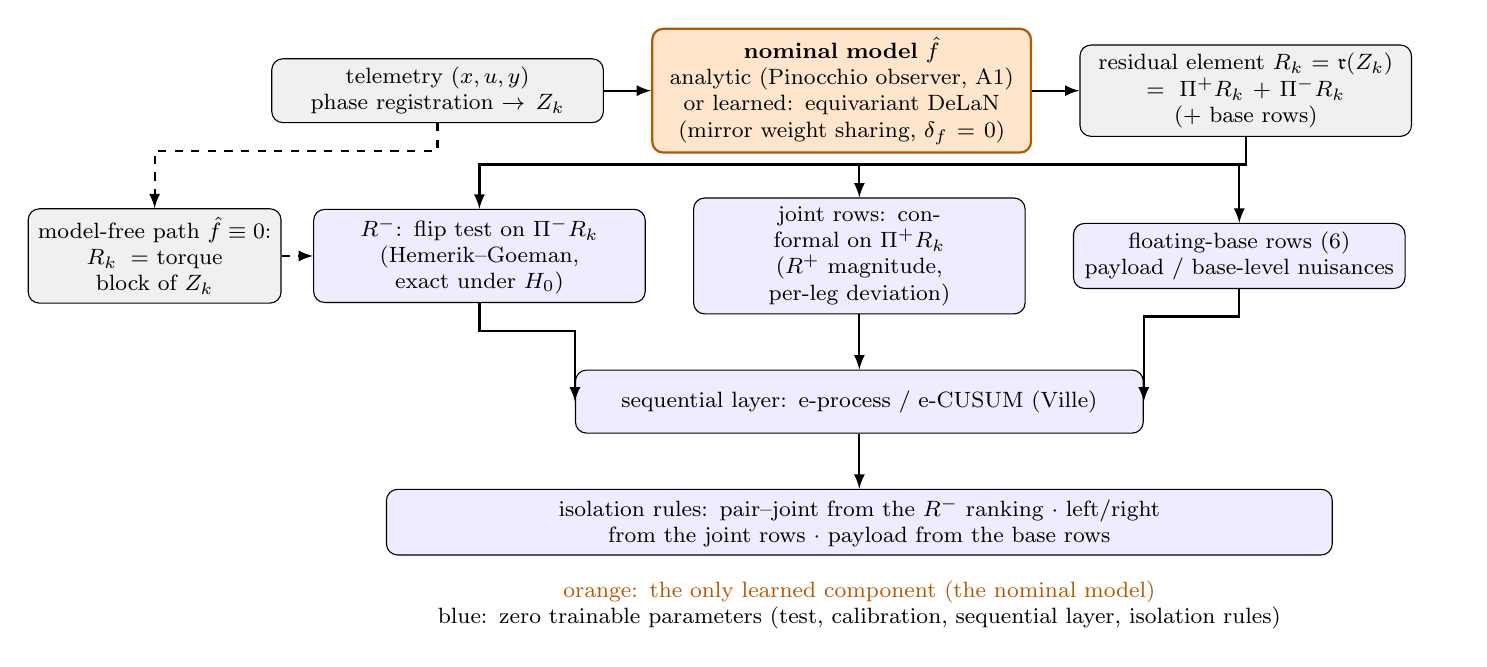
\begin{tikzpicture}[
  font=\footnotesize,
  box/.style={draw, rounded corners, align=center, minimum height=8mm, inner sep=3pt, text width=40mm},
  learn/.style={box, fill=orange!20, draw=orange!70!black, thick, text width=46mm},
  zero/.style={box, fill=blue!7},
  data/.style={box, fill=gray!12},
  arr/.style={-latex, thick},
  node distance=7mm and 6mm]
  \node[data] (tele) {telemetry $(x,u,y)$\\ phase registration $\to Z_k$};
  \node[learn, right=of tele] (model) {\textbf{nominal model $\hat f$}\\ analytic (Pinocchio observer, A1)\\ or learned: equivariant DeLaN\\ (mirror weight sharing, $\delta_f = 0$)};
  \node[data, right=of model] (res) {residual element $R_k = \mathfrak{r}(Z_k)$\\ $=\Pi^{+}R_k + \Pi^{-}R_k$ (+ base rows)};
  \node[zero, below=of model, xshift=-46mm] (rminus) {$R^{-}$: flip test on $\Pi^{-}R_k$\\ (Hemerik--Goeman, exact under $H_0$)};
  \node[zero, right=of rminus] (rplus) {joint rows: conformal on $\Pi^{+}R_k$\\ ($R^{+}$ magnitude, per-leg deviation)};
  \node[zero, right=of rplus] (base) {floating-base rows (6)\\ payload / base-level nuisances};
  \node[zero, below=of rplus, text width=70mm] (seq) {sequential layer: e-process / e-CUSUM (Ville)};
  \node[zero, below=of seq, text width=118mm] (iso) {isolation rules: pair--joint from the $R^{-}$ ranking $\cdot$ left/right from the joint rows $\cdot$ payload from the base rows};
  \node[data, left=4mm of rminus, text width=30mm] (mf) {model-free path $\hat f \equiv 0$:\\ $R_k = $ torque block of $Z_k$};
  \draw[arr] (tele) -- (model);
  \draw[arr] (model) -- (res);
  \draw[arr] (res.south) -- ++(0,-3.5mm) -| (rminus.north);
  \draw[arr] (res.south) -- ++(0,-3.5mm) -| (rplus.north);
  \draw[arr] (res.south) -- ++(0,-3.5mm) -| (base.north);
  \draw[arr] (rminus.south) -- ++(0,-3.5mm) -| (seq.west);
  \draw[arr] (rplus.south) -- (seq.north);
  \draw[arr] (base.south) -- ++(0,-3.5mm) -| (seq.east);
  \draw[arr] (seq) -- (iso);
  \draw[arr, dashed] (tele.south) -- ++(0,-3.5mm) -| (mf.north);
  \draw[arr, dashed] (mf.east) -- (rminus.west);
  \node[below=2mm of iso, align=center, text width=150mm] {\textcolor{orange!70!black}{orange: the only learned component (the nominal model)}\\ blue: zero trainable parameters (test, calibration, sequential layer, isolation rules)};
\end{tikzpicture}}
\caption{Three-channel architecture on the residual data element. The
nominal model is the only learned component (or the analytic observer); the
$R^{-}$ test reads $\Pi^{-}R_k$, the magnitude channel reads $\Pi^{+}R_k$ and
the joint rows, the base rows are the payload channel; the sequential and
isolation layers are fixed rules. The model-free $R^{-}$ of Sprints~1--2 is
the dashed path $\hat f \equiv 0$.}
\label{fig:architecture}
\end{figure}

\subsection{Empirical anchors (Sprint~6, e13; back-filled from the run)}
\label{sec:p2-anchors}

\begin{table}[p]
\centering
\footnotesize
\begin{tabular}{@{}>{\raggedright\arraybackslash}p{0.15\linewidth}>{\raggedright\arraybackslash}p{0.24\linewidth}p{0.55\linewidth}@{}}
\toprule
statement & experiment & status / reading \\
\midrule
Prop.~\ref{prop:residual-h0}, Cor.~\ref{cor:contamination} &
e13b: size of the residual flip test under $H_0$ vs $\delta_f^{(0.95)}$
(plain DeLaN ladder, equivariant ladder, analytic) &
e13b, $R=200$ nominal runs (go2\_urdf\_sym), flip test on the residual element, $\alpha=0.05$, band $[0.02,0.08]$: plain DeLaN residual (uncentred) size $1.00$ at every $\delta_f^{(0.95)} \in \{0.67, 1.47, 3.64, 14.8\}$\,N\,m for $K=60$ and $K=200$; equivariant DeLaN $0.030$--$0.050$ ($K=60$), $0.015$--$0.050$ ($K=200$); analytic residual $0.035/0.060$; raw $Z$ $0.015/0.035$ (URDF world conservative, D005). Naive centring: $1.00$ for every variant (Lemma~\ref{lem:centring}(iii)); $H_0'$ differenced test: $0.00$--$0.045$ for every variant incl.\ the plain $\delta_f^{(0.95)}=14.8$ model (Lemma~\ref{lem:centring}(iv)). Supplement (same seeds, $K\in\{5,10,20,60,200\}$): plain residual size $1.00$ from $K=10$ on for every $\delta_f$ of the ladder; naive centring $0.3/0.7/1.0/1.0$ at $K=10/20/60/200$ (growing with $K/K_{\mathrm{cal}}$ as in (iii)); differenced test in band at all $K$. \textbf{Confirmed} (contamination total already at $K=10$; equivariant/analytic in band or conservative). \\
Prop.~\ref{prop:power-gain} &
e13a: residual vs raw $R^{-}$ power on the low-SNR grid; variance
decomposition $\operatorname{Var}(\Pi^-y)$ vs $\operatorname{Var}(\Pi^-r)$;
Mahalanobis reference &
e13a, $R=50$, e-CUSUM at FAR $0.05$, alarm within 100 cycles: minimal detectable severity (det$\ge 0.9$) residual $R^-$ (analytic / equivariant DeLaN) vs raw $R^-$: bias $0.10$ vs $0.50$\,N\,m (both joints), gain $1-\kappa$ $0.02$ vs $0.05$ (HFE) and $0.02$ vs $0.02$ (KFE), friction $\times 1.5$ vs undetected on the grid; nominal $\operatorname{Var}(\Pi^-r)/\operatorname{Var}(\Pi^-\tau_{\mathrm{cmd}})$ median over rows $0.16$ (analytic), $0.47$ (DeLaN); fault SNR ratio $>1$ in all 22 cells for the analytic residual and in all but the three KFE-gain cells for the DeLaN residual (response term, Remark~\ref{rem:residual-weaker}(i)); Mahalanobis magnitude reference: bias $0.05$, gain $0.01$, friction $\times 1.5$. \textbf{Confirmed} for (a)+(b); the KFE-gain DeLaN cells are the conditional case (c). \\
Cor.~\ref{cor:two-channel} + Thm.~\ref{thm:n1-2} on residuals &
e13c: e04c groups (single / bilateral equal / unequal) with $R^{-}$ on
$\Pi^{-}r$ and $R^{+}$ on $\Pi^{+}r$; three-channel isolation confusion &
e13c, $R=50$, $\kappa$ groups of e04c on the equivariant residual: single --- $R^-$ on $\Pi^-r$ power $1.00$ (e-CUSUM median delay 15 cycles), $R^+$ on $\Pi^+r$ $1.00$ (3 cycles); bilateral equal --- $R^-$ e-process $0.00$, e-CUSUM $0.04$ (FAR level), $\Pi^-$-energy score $0.00$, $\Pi^+$ score $1.00$; unequal --- $R^-$ $1.00$; antisymmetric energy share of the residual signature $0.49 / 0.000 / 0.15$ (raw $Z$: $0.43/0.001/0.06$; a one-joint footprint splits exactly $1/2$--$1/2$). Three-channel isolation ($R=20$, 7 classes incl.\ lateral payload): raw+tracking $0.57$, analytic rows $0.86$, equivariant rows $1.00$. \textbf{Confirmed} (Theorem~\ref{thm:n1-2} verbatim on $R_k$). \\
Prop.~\ref{prop:equiv-delan} &
Block~Q: $\delta_f^{(0.95)}$ and validation RMSE, plain vs equivariant
ladders &
Block~Q (rp012): $\delta_f^{(0.95)}$ of the plain per-leg DeLaN $0.67 / 1.47 / 3.64 / 14.8$\,N\,m at $400$k$/50$k$/10$k$/2$k samples per leg ($\delta_f^{(0.5)}$ $0.21/0.40/1.28/3.44$); mirror-shared model $0$ to the last bit; validation RMSE equivariant vs plain $0.351/0.415$, $0.539/0.559$, $0.80/1.08$, $3.04/2.42$ (2k: 40 gradient steps, seed spread $\pm 0.6$--$0.8$); single template $0.325$; welded trunk $0.573/0.625$. \textbf{Confirmed} ($\delta_f=0$; no accuracy cost except the under-trained 2k cell). \\
\bottomrule
\end{tabular}
\caption{Empirical anchors of Part~2, filled from the e13 run
\texttt{e13-20260815-2334} (rp013) and the Block~Q reports (rp012);
wheeled-M1 anchors (e13d) are pending the M1 world.}
\label{tab:anchors}
\end{table}

% Appendix section of theory Part 0 (input from main.tex). Companion to Definition def:cycle-eps.
\section{Appendix: why the product-kernel defect does not imply Lemma~\ref{lem:eps}}
\label{app:counterexample}

Two cycle-level definitions of the controller defect compete. (P)~The
\emph{product-kernel defect}
$\epsbar{ctrl}^{\mathrm{prod}} := \sup_{x_{0:\Tc-1}} \dtv\bigl(\bigotimes_t
P_{\mathrm{ctrl}}(\cdot\mid x_{t-1},\theta_t),\ \bigotimes_t
P^{\sigma}_{\mathrm{ctrl}}(\cdot\mid x_{t-1},\theta_t)\bigr)$ --- the
equivariance defect of the $\Tc$-fold product kernel with the conditioning
trajectory held \emph{fixed}; (H)~the \emph{closed-loop hybrid displacement}
of \eqref{eq:cycle-eps}. Only (H) bounds the left-hand side of
\eqref{eq:eps-bound}: (P) can be strictly smaller than the closed-loop
displacement, so a lemma stated in (P) would be false.

\paragraph{Setting.}
$\Tc=2$, binary inputs $u_1,u_2\in\{0,1\}$, perfect-memory dynamics
$x_1=u_1$ ($x_0$ fixed), and, with $0<\varepsilon\le\eta<\tfrac12$, nominal
and conjugated controller kernels
$A_1=\mathrm{Bern}(\tfrac12)$, $A_1'=\mathrm{Bern}(\tfrac12+\varepsilon)$,
$A_2(\cdot\mid x)=\mathrm{Bern}(p_x)$, $A_2'(\cdot\mid x)=\mathrm{Bern}(p_x+\varepsilon)$
with $p_1=1-\eta$, $p_0=\eta$. Every per-transition defect equals
$\varepsilon$, so $\eps{ctrl}=\varepsilon$ and the coarse bound
\eqref{eq:linear-bound} reads $\epsbar{ctrl}\le\Tc\,\eps{ctrl}=2\varepsilon$.

\paragraph{What the two definitions compute.}
With $r_t=A_t'/A_t$ and
$D(u_1,x):=\sum_{u_2}A_2(u_2\mid x)\,\lvert 1-r_1(u_1)\,r_2(u_2\mid x)\rvert$,
uniformity of $A_1$ gives
$\epsbar{ctrl}^{\mathrm{prod}}=\max_{x}\tfrac14[D(1,x)+D(0,x)]$ for (P) and
$\Delta_{\mathrm{cl}}=\tfrac14[D(1,x{=}1)+D(0,x{=}0)]$ for (H), because in
the loop branch $u_1$ is evaluated at \emph{its own} state $x_1=u_1$.
Enumerating the four outcomes (verified exactly by brute force):
$D(1,1)=4\varepsilon(1-\eta)+4\varepsilon^2$, $D(0,1)=D(1,0)=2\varepsilon$,
$D(0,0)=4\varepsilon(1-\eta)-4\varepsilon^2$, hence
\[
  \epsbar{ctrl}^{\mathrm{prod}}=\tfrac32\varepsilon-\varepsilon\eta+\varepsilon^2
  \qquad\text{versus}\qquad
  \Delta_{\mathrm{cl}}=2\varepsilon(1-\eta)\;>\;\epsbar{ctrl}^{\mathrm{prod}}
  \quad\text{whenever }\eta+\varepsilon<\tfrac12
\]
(e.g.\ $\varepsilon=\eta=0.1$: $0.150$ versus $0.180$, linear bound $0.20$;
$\varepsilon=\eta=0.01$: $0.0150$ versus $0.0198$, bound $0.02$).

\paragraph{Why the closed loop exceeds the product defect.}
$\Delta_{\mathrm{cl}}$ is a \emph{mixture of branch-wise maxima},
$\tfrac14\sum_{u_1}\max_x D(u_1,x)$, whereas (P) is the \emph{maximum of the
mixture}, $\max_x\tfrac14\sum_{u_1}D(u_1,x)$; the former dominates, strictly
when the worst-case conditioning differs across branches --- here the step-2
defect that aligns with the step-1 likelihood ratio sits at $x{=}1$ for
$u_1{=}1$ and at $x{=}0$ for $u_1{=}0$, and the loop delivers exactly that
state to each branch. Holding the trajectory fixed in (P) discards the
input--state correlation that makes defects add up. As $\eta\to0$,
$\Delta_{\mathrm{cl}}\to2\varepsilon=\Tc\,\eps{ctrl}$: the coarse linear
bound is attained, consistent with Remark~\ref{rem:linear}. Part~0 therefore
defines $\epsbar{\bullet}$ as the closed-loop hybrid displacement (H), for
which Lemma~\ref{lem:eps} is a triangle inequality by construction, and treats
(P)-type quantities only as what the state-matched audits estimate per
transition.


\bibliographystyle{ieeetr}
\bibliography{references}

\end{document}
